\documentclass[
  man,
  longtable,
  nolmodern,
  notxfonts,
  notimes,
  colorlinks=true,linkcolor=blue,citecolor=blue,urlcolor=blue]{apa7}

\usepackage{amsmath}
\usepackage{amssymb}




\RequirePackage{longtable}
\RequirePackage{threeparttablex}

\makeatletter
\renewcommand{\paragraph}{\@startsection{paragraph}{4}{\parindent}%
	{0\baselineskip \@plus 0.2ex \@minus 0.2ex}%
	{-.5em}%
	{\normalfont\normalsize\bfseries\typesectitle}}

\renewcommand{\subparagraph}[1]{\@startsection{subparagraph}{5}{0.5em}%
	{0\baselineskip \@plus 0.2ex \@minus 0.2ex}%
	{-\z@\relax}%
	{\normalfont\normalsize\bfseries\itshape\hspace{\parindent}{#1}\textit{\addperi}}{\relax}}
\makeatother




\usepackage{longtable, booktabs, multirow, multicol, colortbl, hhline, caption, array, float, xpatch}
\usepackage{subcaption}


\renewcommand\thesubfigure{\Alph{subfigure}}
\setcounter{topnumber}{2}
\setcounter{bottomnumber}{2}
\setcounter{totalnumber}{4}
\renewcommand{\topfraction}{0.85}
\renewcommand{\bottomfraction}{0.85}
\renewcommand{\textfraction}{0.15}
\renewcommand{\floatpagefraction}{0.7}

\usepackage{tcolorbox}
\tcbuselibrary{listings,theorems, breakable, skins}
\usepackage{fontawesome5}

\definecolor{quarto-callout-color}{HTML}{909090}
\definecolor{quarto-callout-note-color}{HTML}{0758E5}
\definecolor{quarto-callout-important-color}{HTML}{CC1914}
\definecolor{quarto-callout-warning-color}{HTML}{EB9113}
\definecolor{quarto-callout-tip-color}{HTML}{00A047}
\definecolor{quarto-callout-caution-color}{HTML}{FC5300}
\definecolor{quarto-callout-color-frame}{HTML}{ACACAC}
\definecolor{quarto-callout-note-color-frame}{HTML}{4582EC}
\definecolor{quarto-callout-important-color-frame}{HTML}{D9534F}
\definecolor{quarto-callout-warning-color-frame}{HTML}{F0AD4E}
\definecolor{quarto-callout-tip-color-frame}{HTML}{02B875}
\definecolor{quarto-callout-caution-color-frame}{HTML}{FD7E14}

%\newlength\Oldarrayrulewidth
%\newlength\Oldtabcolsep


\usepackage{hyperref}




\providecommand{\tightlist}{%
  \setlength{\itemsep}{0pt}\setlength{\parskip}{0pt}}
\usepackage{longtable,booktabs,array}
\usepackage{calc} % for calculating minipage widths
% Correct order of tables after \paragraph or \subparagraph
\usepackage{etoolbox}
\makeatletter
\patchcmd\longtable{\par}{\if@noskipsec\mbox{}\fi\par}{}{}
\makeatother
% Allow footnotes in longtable head/foot
\IfFileExists{footnotehyper.sty}{\usepackage{footnotehyper}}{\usepackage{footnote}}
\makesavenoteenv{longtable}

\usepackage{graphicx}
\makeatletter
\newsavebox\pandoc@box
\newcommand*\pandocbounded[1]{% scales image to fit in text height/width
  \sbox\pandoc@box{#1}%
  \Gscale@div\@tempa{\textheight}{\dimexpr\ht\pandoc@box+\dp\pandoc@box\relax}%
  \Gscale@div\@tempb{\linewidth}{\wd\pandoc@box}%
  \ifdim\@tempb\p@<\@tempa\p@\let\@tempa\@tempb\fi% select the smaller of both
  \ifdim\@tempa\p@<\p@\scalebox{\@tempa}{\usebox\pandoc@box}%
  \else\usebox{\pandoc@box}%
  \fi%
}
% Set default figure placement to htbp
\def\fps@figure{htbp}
\makeatother


% definitions for citeproc citations
\NewDocumentCommand\citeproctext{}{}
\NewDocumentCommand\citeproc{mm}{%
  \begingroup\def\citeproctext{#2}\cite{#1}\endgroup}
\makeatletter
 % allow citations to break across lines
 \let\@cite@ofmt\@firstofone
 % avoid brackets around text for \cite:
 \def\@biblabel#1{}
 \def\@cite#1#2{{#1\if@tempswa , #2\fi}}
\makeatother
\newlength{\cslhangindent}
\setlength{\cslhangindent}{1.5em}
\newlength{\csllabelwidth}
\setlength{\csllabelwidth}{3em}
\newenvironment{CSLReferences}[2] % #1 hanging-indent, #2 entry-spacing
 {\begin{list}{}{%
  \setlength{\itemindent}{0pt}
  \setlength{\leftmargin}{0pt}
  \setlength{\parsep}{0pt}
  % turn on hanging indent if param 1 is 1
  \ifodd #1
   \setlength{\leftmargin}{\cslhangindent}
   \setlength{\itemindent}{-1\cslhangindent}
  \fi
  % set entry spacing
  \setlength{\itemsep}{#2\baselineskip}}}
 {\end{list}}
\usepackage{calc}
\newcommand{\CSLBlock}[1]{\hfill\break\parbox[t]{\linewidth}{\strut\ignorespaces#1\strut}}
\newcommand{\CSLLeftMargin}[1]{\parbox[t]{\csllabelwidth}{\strut#1\strut}}
\newcommand{\CSLRightInline}[1]{\parbox[t]{\linewidth - \csllabelwidth}{\strut#1\strut}}
\newcommand{\CSLIndent}[1]{\hspace{\cslhangindent}#1}





\usepackage{newtx}

\defaultfontfeatures{Scale=MatchLowercase}
\defaultfontfeatures[\rmfamily]{Ligatures=TeX,Scale=1}





\title{The Link Function Problem in Psychological Interaction Testing}


\shorttitle{Link Functions and Interactions}


\usepackage{etoolbox}









\authorsnames[{1},{2},{1},{1},{1}]{Enrico Toffalini,Filippo
Gambarota,Laura Sità,Tommaso Feraco,Margherita Calderan}







\authorsaffiliations{
{Department of General Psychology, University of Padova},{Department of
Developmental Psychology and Socialization, University of Padova}}




\leftheader{Toffalini, Gambarota, Sità, Feraco and Calderan}



\abstract{Interaction tests are common in psychology, but an interaction
claim is not defined by a product term alone. It also depends on the
scale on which additivity is assumed. We reframe this scale problem in
the GLM language of outcome family and link function: the family
describes the response, whereas the link defines the scale on which no
interaction is assumed. We first report a preregistered descriptive
review of recent psychological articles, showing that interaction tests
are common and that family, link, and scale-of-additivity choices are
often implicit, especially for bounded, discrete, ordinal, accuracy, and
sum-score outcomes. We then develop a link-centered framework that
distinguishes wrong-family, wrong-link, and measurement-metric problems,
and separates interactions on the linear predictor scale from
interactions on the observed response scale. Worked examples and
simulations focus on forced-choice accuracy with a non-zero chance
floor, sum scores, and within-family link choices such as logit versus
probit. The simulations show that plausible but inadequate links can
turn additive main-effect structures on one scale into statistically
significant pseudo-interactions on another. A diagnostic simulation
shows that residual checks, link checks, and AIC comparisons may help,
but they do not by themselves decide which scale is right for the
scientific interaction claim. We argue that interaction claims are often
underspecified unless researchers state, justify, and probe the scale on
which no interaction is assumed. }

\keywords{interactions, moderation, generalized linear models, link
functions, model misspecification}

\authornote{\par{\addORCIDlink{Enrico
Toffalini}{0000-0002-1404-5133}}\par{\addORCIDlink{Filippo
Gambarota}{0000-0002-6666-1747}}\par{\addORCIDlink{Laura
Sità}{0009-0000-6017-9979}}\par{\addORCIDlink{Tommaso
Feraco}{0000-0002-8920-5330}}\par{\addORCIDlink{Margherita
Calderan}{0009-0005-5668-5162}} 
\par{ }
\par{       }
\par{Correspondence concerning this article should be addressed
to Enrico Toffalini, Department of General Psychology, University of
Padova, Via Venezia
8, Padova 35131, Italy, Email: \href{mailto:enrico.toffalini@unipd.it}{enrico.toffalini@unipd.it}}
}

\makeatletter
\let\endoldlt\endlongtable
\def\endlongtable{
\hline
\endoldlt
}
\makeatother
\RequirePackage{longtable}
\DeclareDelayedFloatFlavor{longtable}{table}

\urlstyle{same}



\makeatletter
\@ifpackageloaded{tcolorbox}{}{\usepackage[skins,breakable]{tcolorbox}}
\@ifpackageloaded{fontawesome5}{}{\usepackage{fontawesome5}}
\definecolor{quarto-callout-color}{HTML}{909090}
\definecolor{quarto-callout-note-color}{HTML}{0758E5}
\definecolor{quarto-callout-important-color}{HTML}{CC1914}
\definecolor{quarto-callout-warning-color}{HTML}{EB9113}
\definecolor{quarto-callout-tip-color}{HTML}{00A047}
\definecolor{quarto-callout-caution-color}{HTML}{FC5300}
\definecolor{quarto-callout-color-frame}{HTML}{acacac}
\definecolor{quarto-callout-note-color-frame}{HTML}{4582ec}
\definecolor{quarto-callout-important-color-frame}{HTML}{d9534f}
\definecolor{quarto-callout-warning-color-frame}{HTML}{f0ad4e}
\definecolor{quarto-callout-tip-color-frame}{HTML}{02b875}
\definecolor{quarto-callout-caution-color-frame}{HTML}{fd7e14}
\makeatother
\makeatletter
\@ifpackageloaded{caption}{}{\usepackage{caption}}
\AtBeginDocument{%
\ifdefined\contentsname
  \renewcommand*\contentsname{Table of contents}
\else
  \newcommand\contentsname{Table of contents}
\fi
\ifdefined\listfigurename
  \renewcommand*\listfigurename{List of Figures}
\else
  \newcommand\listfigurename{List of Figures}
\fi
\ifdefined\listtablename
  \renewcommand*\listtablename{List of Tables}
\else
  \newcommand\listtablename{List of Tables}
\fi
\ifdefined\figurename
  \renewcommand*\figurename{Figure}
\else
  \newcommand\figurename{Figure}
\fi
\ifdefined\tablename
  \renewcommand*\tablename{Table}
\else
  \newcommand\tablename{Table}
\fi
}
\@ifpackageloaded{float}{}{\usepackage{float}}
\floatstyle{ruled}
\@ifundefined{c@chapter}{\newfloat{codelisting}{h}{lop}}{\newfloat{codelisting}{h}{lop}[chapter]}
\floatname{codelisting}{Listing}
\newcommand*\listoflistings{\listof{codelisting}{List of Listings}}
\makeatother
\makeatletter
\makeatother
\makeatletter
\@ifpackageloaded{caption}{}{\usepackage{caption}}
\@ifpackageloaded{subcaption}{}{\usepackage{subcaption}}
\makeatother

% From https://tex.stackexchange.com/a/645996/211326
%%% apa7 doesn't want to add appendix section titles in the toc
%%% let's make it do it
\makeatletter
\xpatchcmd{\appendix}
  {\par}
  {\addcontentsline{toc}{section}{\@currentlabelname}\par}
  {}{}
\makeatother

%% Disable longtable counter
%% https://tex.stackexchange.com/a/248395/211326

\usepackage{etoolbox}

\makeatletter
\patchcmd{\LT@caption}
  {\bgroup}
  {\bgroup\global\LTpatch@captiontrue}
  {}{}
\patchcmd{\longtable}
  {\par}
  {\par\global\LTpatch@captionfalse}
  {}{}
\apptocmd{\endlongtable}
  {\ifLTpatch@caption\else\addtocounter{table}{-1}\fi}
  {}{}
\newif\ifLTpatch@caption
\makeatother

\begin{document}

\maketitle




\setlength\LTleft{0pt}




Psychological theories often test whether the effect of one variable
depends on another. Stress may impair performance more strongly among
people with high anxiety. A treatment may help some participants more
than others. A developmental difference may be large at one age and
small at another. These are interaction claims: claims about moderation,
boundary conditions, and heterogeneous effects. In practice, testing
such claims has become almost a routine step after main effects have
been examined. This routine use is understandable, because interactions
often express important theoretical ideas. Yet an interaction claim
should not be interpreted automatically from the presence or absence of
a product term (\citeproc{ref-rimpler2026}{Rimpler et al., 2026};
\citeproc{ref-rohrer2021}{Rohrer \& Arslan, 2021}).

Statistically, many interaction claims can be understood as claims about
a difference between differences. Does the treatment-control difference
change across groups? Does the age-related difference differ between
populations? Does the effect of task difficulty vary as anxiety
increases? While this formulation sounds intuitive, it hides a crucial
assumption. An interaction is a difference between differences, but
whether two differences are equal depends on the scale on which those
differences are expressed.

The scale problem has been recognized for a long time. Loftus argued
that interactions involving response probabilities are meaningful only
relative to an assumed mapping between the observed response and the
theoretical component of interest (\citeproc{ref-loftus1978}{Loftus,
1978}). Cox treated interaction as a statistical concept tied to model
formulation, transformation, and interpretation
(\citeproc{ref-cox1984}{Cox, 1984}). Wagenmakers and colleagues later
emphasized the distinction between removable and nonremovable
interactions, showing that some interactions depend on the measurement
scale and therefore do not support unambiguous conclusions about latent
psychological processes (\citeproc{ref-wagenmakers2012}{Wagenmakers et
al., 2012}). Lubinski and Humphreys illustrated how apparently
substantive moderator effects can arise from model specification choices
rather than real psychological synergy
(\citeproc{ref-lubinski1990}{Lubinski \& Humphreys, 1990}). More
recently, Rohrer and Arslan argued that interaction tests can provide
precise answers to vague questions when researchers do not specify the
estimand, scale, or substantive meaning of the interaction
(\citeproc{ref-rohrer2021}{Rohrer \& Arslan, 2021}).

In psychology, this scale problem often has a measurement origin.
Researchers usually reason about constructs such as ability, symptom
severity, attitude strength, processing efficiency, or others as if they
were continuous underlying dimensions. Most psychological dimensions may
indeed be treated as smooth and roughly Gaussian, because they plausibly
reflect many small sources of variation. If such processes were observed
directly on an interval scale, a Gaussian identity model might often be
a reasonable solution. But psychological phenomena are rarely observed
directly. They are observed indirectly through tasks, items, ratings,
counts, accuracies, and summed responses. These observations impose
bounds, thresholds, discreteness, floors, ceilings, and chance levels.
The link-function problem is one formal expression of this broader
psychometric problem: the model must say how an additive structure on
one scale is mapped onto the scale on which the data are observed.

A related literature has sharpened the problem for modern psychological
data. Domingue and colleagues showed that misspecifying the outcome
model can produce bias and false discoveries in interaction analyses,
especially when outcomes are binary, count, or censored
(\citeproc{ref-domingue2024}{Domingue et al., 2024}). McCabe and
colleagues showed that, in generalized linear models (GLMs) for
probabilities and counts, product-term coefficients are not generally
equal to interaction effects on the response scale
(\citeproc{ref-mccabe2022}{McCabe et al., 2022}). Work on nonlinear
probability models reaches the same practical conclusion: interaction
effects should often be evaluated as conditional marginal effects or
response-scale contrasts, not as product coefficients alone
(\citeproc{ref-ainorton2003}{Ai \& Norton, 2003};
\citeproc{ref-mize2019}{Mize, 2019}). More broadly, estimand-centered
approaches recommend treating models as tools for generating
substantively meaningful quantities rather than interpreting
coefficients mechanically (\citeproc{ref-rohrer2026}{Rohrer \&
Arel-Bundock, 2026}). Rimpler and colleagues further emphasized that a
theoretical claim of conditionality does not automatically imply that
the correct statistical representation is a multiplicative product term
(\citeproc{ref-rimpler2026}{Rimpler et al., 2026}). Together, these
contributions show that interaction testing is not only a matter of
adding the right-hand-side product term to a regression equation.

The present paper focuses on one specific part of this broader problem:
the role of the link function in GLM interaction testing. We do not
claim that scale dependence of interactions is new
(\citeproc{ref-cox1984}{Cox, 1984}; \citeproc{ref-loftus1978}{Loftus,
1978}; \citeproc{ref-wagenmakers2012}{Wagenmakers et al., 2012}), or
that product terms in GLMs can be read directly as response-scale
interactions (\citeproc{ref-ainorton2003}{Ai \& Norton, 2003};
\citeproc{ref-mccabe2022}{McCabe et al., 2022};
\citeproc{ref-mize2019}{Mize, 2019}). Our contribution is narrower. We
translate the scale-dependence problem into the GLM distinction between
outcome family and link function, show that link and scale choices are
often implicit in recent psychological interaction tests, develop
psychology-specific cases in which plausible links imply different
no-interaction baselines, and use simulations to show how inadequate
links can generate pseudo-interactions under realistic conditions.

Choosing an appropriate family is therefore necessary, but not
sufficient, for appropriate interaction testing. Two models can respect
the same outcome family while defining different no-interaction
baselines. For response times, for example, a Gamma family may be
plausible because the outcome is positive, continuous, and right-skewed.
Yet \texttt{Gamma(link\ =\ "log")} assumes additivity in log mean
response times, which corresponds to proportional change on the
millisecond scale, whereas \texttt{Gamma(link\ =\ "inverse")}, the
canonical link, assumes additivity in inverse mean response times.
Neither choice is automatically correct. The relevant question is
whether the scientific claim concerns proportional change, reciprocal
change, absolute change, or some other scale. Link misspecification can
affect likelihood-based inference in GLMs and GLMMs
(\citeproc{ref-czadosantner1992}{Czado \& Santner, 1992};
\citeproc{ref-yuhuang2019}{Yu \& Huang, 2019}).

The same logic applies to binary and accuracy data, which are frequently
reported in psychological research. A binomial family may correctly
represent the sampling process of correct and incorrect responses, but
the link still defines the scale of additivity. A standard logit link
maps the linear predictor to the full 0-to-1 probability range, and a
probit link makes a similar but not identical mapping, with different
curvature especially away from the middle of the probability scale. In a
two-alternative forced-choice task, however, the theoretically
meaningful lower bound may be chance performance, that is, \(0.50\). A
chance-corrected link can encode this lower asymptote directly. Thus,
the distinction is not only between linear models and GLMs. It is also
across plausible links within a generally appropriate family.

\begin{figure}

\caption{\label{fig-family-link-distinction}Same outcome family,
different link functions. The grey construction lines are drawn from a
target link: the chance-corrected logit in Panel A and the log link in
Panel B. Vertical grey lines mark equal intervals on the target-link
linear predictor scale. Horizontal grey lines show where those equally
spaced target-link values fall on the observed response scale. The key
point is that equal intervals on one link scale do not remain equal
intervals under another link. Thus, models with the same outcome family
can imply different no-interaction baselines, even when their fitted
curves look similar over the observed range.}

\centering{

\pandocbounded{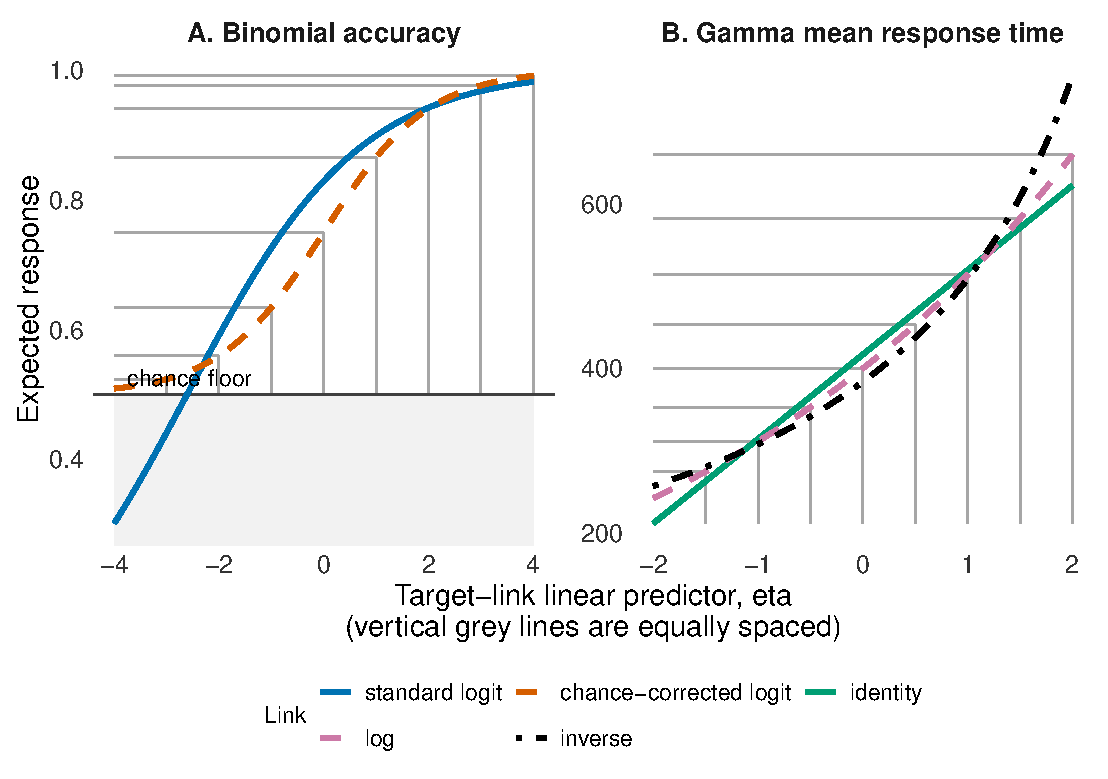
\includegraphics[keepaspectratio]{paper_files/figure-pdf/fig-family-link-distinction-1.pdf}}

}

\end{figure}%

Figure~\ref{fig-family-link-distinction} shows why link choice is a
scale choice, not only a curve-fitting choice. In each panel, the grey
construction lines are anchored to a target link: the chance-corrected
logit for forced-choice accuracy and the log link for Gamma mean
response times. Equal steps on the target-link scale map to unequal
steps on any other scale. Conversely, the same observed response values
would not be equally spaced on an alternative link scale. Floor and
ceiling effects are the most visible version of this problem, because
the response scale has almost no room left to move. But the same logic
is not limited to the endpoints: when the inverse link is nonlinear, the
amount of response-scale change implied by the same link-scale effect
varies across the scale. This is the central reason why link choice
matters for interactions. A data-generating process without a product
term is matched by an additive model only on the scale defined by the
correct link. When another plausible link is used, the same
response-scale pattern can imply a different no-interaction baseline and
therefore a different moderation claim.

Figure~\ref{fig-motivating-example} uses a simulated two-alternative
forced-choice accuracy dataset as an illustrative example. Each
participant completes 50 trials, and the outcome is the proportion
correct. The predictors are age and group. The data-generating model
includes an age effect and a group effect, but no age-by-group term on
the chance-corrected logit scale, the scale on which the task has a
\(0.50\) chance floor. The figure illustrates how the same data can
apparently support different moderation claims when fitted models define
different no-interaction baselines (\citeproc{ref-cox1984}{Cox, 1984};
\citeproc{ref-domingue2024}{Domingue et al., 2024};
\citeproc{ref-loftus1978}{Loftus, 1978};
\citeproc{ref-mccabe2022}{McCabe et al., 2022}), that is, when they use
different link functions.

\begin{figure}

\caption{\label{fig-motivating-example}Same data, different link
functions. Data were simulated from a 2-alternative forced-choice
accuracy task with 50 trials per participant and a 0.50 chance floor.
The data-generating model included age and group effects, but no
age-by-group interaction on the chance-corrected 2-AFC logit scale.
Panel A shows the true response-scale pattern implied by that model.
Panel B shows one simulated dataset. Panel C fits the same data with
three models. The Gaussian identity model is simple and interpretable on
the observed accuracy scale, but it can produce predictions outside the
0-to-1 range and ignores the binomial sampling process. The standard
binomial logit/probit model, shown here with a logit link, respects the
binomial process and the 0-to-1 range, but assumes a lower asymptote at
0. The chance-corrected binomial link incorporates the task's chance
floor. The question is which scale defines the scientific null
hypothesis of no moderation.}

\centering{

\pandocbounded{
\includegraphics[keepaspectratio]{figs/fig1-motivating-example.pdf}}

}

\end{figure}%

This does not mean that all interactions are artifacts, or that scale
choices make any interaction claim arbitrary. Some interactions are
robust across any link function {[}e.g., non-removable or crossover
interactions; Loftus (\citeproc{ref-loftus1978}{1978}); Cox
(\citeproc{ref-cox1984}{1984}); Wagenmakers et al.
(\citeproc{ref-wagenmakers2012}{2012}){]}. The problem is that many
interaction claims are underspecified unless researchers state which
scale defines additivity, whether the reported interaction is on the
linear predictor scale or the observed response scale, and whether
alternative plausible links lead to the same substantive conclusion. In
this sense, link choice is not just a technical detail, but it becomes
part of the scientific claim.

The sections below develop this argument in a compact order. The review
first shows why the problem matters for current reporting practice. The
framework then separates outcome family, link function, and measurement
metric, and distinguishes link-scale from response-scale interactions.
The applied sections focus on three cases in which these distinctions
can change moderation claims: forced-choice accuracy with a non-zero
chance floor, sum scores, and within-family link choice. The simulations
then quantify when these choices can generate pseudo-interactions, and
the diagnostic example asks whether standard checks detect the same
misspecification.

The paper first looks at current practice. A preregistered descriptive
review of recent psychological articles shows how often interaction
tests are used and how often family, link, and scale choices are made
explicit. The next section defines the link-function problem,
distinguishing interactions on the linear predictor scale from
interactions on the observed response scale. The central applied
sections focus on three cases in which link assumptions can change
moderation claims: forced-choice accuracy with a non-zero chance floor,
sum scores, and within-family link choice. The simulation studies
quantify when wrong or inadequate links generate pseudo-interactions,
and one diagnostic scenario shows what standard checks can and cannot
detect. The paper closes with a minimal workflow for link-aware
interaction testing in psychological research.

\section{Current Practice in Psychological Interaction Testing: A
Preregistered
Review}\label{current-practice-in-psychological-interaction-testing-a-preregistered-review}

\subsection{Why This Review Matters}\label{why-this-review-matters}

Do these issues matter for current psychological practice? This question
motivated our preregistered descriptive review. The review examined
whether the link-function problem is relevant to the kinds of
interaction analyses that psychologists actually report. If interaction
tests were rare, or if researchers usually stated the outcome family,
link function, and scale of additivity, the problem would be less
pressing. If, instead, interaction tests are common and these modeling
choices are often implicit, then many moderation claims are difficult to
evaluate, because the no-interaction baseline is not fully specified.

The present review is not an audit of individual articles. We did not
aim to decide whether each reported interaction was right or wrong, or
whether it was removable or nonremovable. Such judgments often require
more information than published reports provide, such as detailed
interaction plots, complete model coefficients, the assumed measurement
scale, the link function, or the substantive scale on which the
interaction was meant to hold. Although this distinction is central in
the classical scale-dependence literature (\citeproc{ref-cox1984}{Cox,
1984}; \citeproc{ref-loftus1978}{Loftus, 1978};
\citeproc{ref-wagenmakers2012}{Wagenmakers et al., 2012}), we did not
systematically code it because it could not be reconstructed reliably
from many published reports. Instead, we treated the review as a
description of reported practice. We focused on what could be observed
from the articles: how often interaction tests were used, whether link
functions were stated explicitly, and how often the outcomes were of a
kind for which identity-link additivity is not an obvious default. The
broader implication is that many interaction claims are partly
underspecified when the outcome family, link function, and scale of
additivity are left implicit. Making these choices explicit is part of
good quantitative reporting, because readers need enough information to
understand which model was fitted and which kind of interaction was
tested (\citeproc{ref-mustillo2018}{Mustillo et al., 2018}).

\subsection{Review Method}\label{review-method}

The review protocol was preregistered before the records were screened,
at: xxxxxxxxxxxxxx. We specified a descriptive review of recently
published psychological research articles, with four primary goals:
estimating how often empirical articles test interactions, how often
interaction-testing articles use non-identity links, how often the link
function is explicitly reported, and which response-variable types are
used in interaction analyses. The protocol also stated that the review
was not intended to be an exhaustive systematic review of psychology as
a whole, but a targeted estimate of current practice in selected
journals.

Sampled articles were recent publications, all from 2024, in five
prominent journals: \emph{Psychological Science}, \emph{Journal of
Experimental Psychology: General}, \emph{Journal of Personality and
Social Psychology}, \emph{Developmental Science}, and
\emph{Psychological Medicine}. These journals were pre-specified by the
authors to cover different areas of psychology. Eligible articles were
empirical articles presenting original psychological research. Reviews,
meta-analyses, editorials, theoretical articles without empirical data,
qualitative-only articles, replication studies, and psychometric
validation studies were excluded. After preregistration, we also
excluded articles in which the relevant tests were conducted only at the
latent-variable level, or in which the empirical analyses relied only on
structural equation models (SEM). This decision kept the review focused
on observed outcomes analyzed with regression, ANOVA, or GLM-like
models. SEM is relevant to the broader issue because it can make the
measurement model explicit and may therefore help address some scale
problems. At the same time, SEM raises additional questions about links,
thresholds, loadings, and latent-response metrics that would require a
different coding scheme and are beyond the scope of the present review.
Articles were then coded in detail if they tested at least one
interaction effect, either through statistical modeling or analysis of
variance.

For each interaction-testing article, coders recorded whether at least
one tested interaction used a non-identity link function, whether the
link function was explicitly reported, whether at least one interaction
was analyzed with an identity link when another link appeared more
appropriate given the outcome, whether at least one such interaction was
statistically significant or interpreted analogously, and which
response-variable types were analyzed. The protocol specified
descriptive summaries, including proportions and Wilson 95\% confidence
intervals for Boolean variables. The full review protocol, coding
definitions, and extended descriptive tables are reported in the
Supplement.

\subsection{Review Findings}\label{review-findings}

The review identified 331 eligible empirical articles. Interaction
testing was common: 200 of these articles tested at least one
interaction, corresponding to 60.4\%, 95\% CI {[}55.1, 65.5{]}. Among
the 200 interaction-testing articles, 58 used at least one non-identity
link function, 29\%, 95\% CI {[}23.2, 35.6{]}, and only 46 explicitly
reported the link function, 23\%, 95\% CI {[}17.7, 29.3{]}. Thus, in
most interaction-testing articles, the link function was either identity
by default, not reported explicitly, or not foregrounded as part of the
interaction claim.

A large proportion of interaction-testing articles involved outcomes for
which identity-link additivity required explicit justification. Among
the 200 articles testing interactions, 144 were coded as including at
least one identity-link analysis for which another link appeared
plausibly relevant given the reported outcome, 72\%, 95\% CI {[}65.4,
77.8{]}. This code should be interpreted cautiously. It does not show
that the fitted model was wrong, or that the specific interaction claim
was false. It shows that the scale of additivity was not self-evident
from the outcome and model description. This is the same broad concern
raised by work on outcome-model mismatch and metric assumptions in
interaction testing (\citeproc{ref-domingue2024}{Domingue et al., 2024};
\citeproc{ref-liddellkruschke2018}{Liddell \& Kruschke, 2018}). Among
these 144 cases, 124 reported at least one statistically significant
interaction, 86.1\%, 95\% CI {[}79.5, 90.8{]}.
Table~\ref{tbl-current-practice} summarizes these descriptive results.

\begin{table}

{\caption{{Descriptive summary of the preregistered review of
interaction testing and link-function
reporting.}{\label{tbl-current-practice}}}
\vspace{-20pt}}

\begin{longtable}[]{@{}
  >{\raggedright\arraybackslash}p{(\linewidth - 8\tabcolsep) * \real{0.6970}}
  >{\raggedleft\arraybackslash}p{(\linewidth - 8\tabcolsep) * \real{0.0303}}
  >{\raggedleft\arraybackslash}p{(\linewidth - 8\tabcolsep) * \real{0.0909}}
  >{\raggedleft\arraybackslash}p{(\linewidth - 8\tabcolsep) * \real{0.0606}}
  >{\raggedleft\arraybackslash}p{(\linewidth - 8\tabcolsep) * \real{0.1212}}@{}}
\toprule\noalign{}
\begin{minipage}[b]{\linewidth}\raggedright
Quantity
\end{minipage} & \begin{minipage}[b]{\linewidth}\raggedleft
n
\end{minipage} & \begin{minipage}[b]{\linewidth}\raggedleft
Denominator
\end{minipage} & \begin{minipage}[b]{\linewidth}\raggedleft
Percent
\end{minipage} & \begin{minipage}[b]{\linewidth}\raggedleft
95\% CI
\end{minipage} \\
\midrule\noalign{}
\endhead
\bottomrule\noalign{}
\endlastfoot
Eligible empirical articles reviewed & 331 & 331 & 100.0\% & {[}98.9\%,
100.0\%{]} \\
Articles testing at least one interaction & 200 & 331 & 60.4\% &
{[}55.1\%, 65.5\%{]} \\
Interaction-testing articles using a non-identity link & 58 & 200 &
29.0\% & {[}23.2\%, 35.6\%{]} \\
Interaction-testing articles explicitly reporting the link function & 46
& 200 & 23.0\% & {[}17.7\%, 29.3\%{]} \\
Interaction-testing articles with identity-link analyses requiring scale
justification & 144 & 200 & 72.0\% & {[}65.4\%, 77.8\%{]} \\
Identity-link cases requiring scale justification with at least one
significant interaction & 124 & 144 & 86.1\% & {[}79.5\%, 90.8\%{]} \\
\end{longtable}

\end{table}

The outcomes used in interaction analyses were heterogeneous. The most
common broad, non-exclusive categories were binary, accuracy, or
proportion outcomes (86 articles), sum scores or composites (77
articles), ordinal, Likert, or rating outcomes (49 articles), response
times or durations (29 articles), and counts or error counts (12
articles). This heterogeneity matters because the identity link has
different implications across outcome types. For some approximately
continuous outcomes, additivity on the observed scale may be a
defensible target. For bounded, discrete, ordinal, chance-constrained,
or heavily transformed outcomes, however, additivity on the observed
scale is an assumption that should usually be stated and examined. This
is especially clear for ordinal and Likert-type outcomes, where treating
ordered categories as metric can affect estimates, error rates, and
interaction conclusions (\citeproc{ref-burknervuorre2019}{Bürkner \&
Vuorre, 2019}; \citeproc{ref-liddellkruschke2018}{Liddell \& Kruschke,
2018}).

\begin{table}

{\caption{{Broad response-variable categories in interaction-testing
articles. Categories are non-exclusive, so one article can contribute to
more than one row.}{\label{tbl-review-outcome-types}}}
\vspace{-20pt}}

\begin{longtable}[]{@{}lrrr@{}}
\toprule\noalign{}
Outcome type & n & Denominator & Percent \\
\midrule\noalign{}
\endhead
\bottomrule\noalign{}
\endlastfoot
Binary / accuracy / proportions & 86 & 200 & 43.0\% \\
Sum scores / composites & 77 & 200 & 38.5\% \\
Ordinal / Likert / ratings & 49 & 200 & 24.5\% \\
Response times / durations & 29 & 200 & 14.5\% \\
Neural / physiological measures & 23 & 200 & 11.5\% \\
Difference / distance scores & 21 & 200 & 10.5\% \\
Counts / error counts & 12 & 200 & 6.0\% \\
Correlations / associations & 8 & 200 & 4.0\% \\
\end{longtable}

\end{table}

\subsection{What the Review Shows, and What It Does Not
Show}\label{what-the-review-shows-and-what-it-does-not-show}

The review shows that interaction testing is a routine part of current
psychological practice, and that many interaction claims are made in
settings where the scale of additivity is not trivial. It also shows
that link functions are rarely made explicit. This combination is the
key empirical result. If the link function defines the scale on which
effects are assumed to add, then an implicit link function implies an
implicit no-interaction baseline.

The review does not show that the coded articles reached wrong
conclusions. Some identity-link analyses may have been reasonable
approximations. Some interaction claims may be robust across plausible
links. Some authors may have intentionally targeted observed-scale
differences, even if this was not stated in link-function language. The
review also does not classify individual interactions as removable or
nonremovable, because doing so would often require stronger information
than the published report provides. The descriptive result is more
modest, but still important: many published interaction claims are
underspecified from the reader's perspective because the family, link,
and scale of additivity are not made sufficiently explicit.

The next section turns this reporting issue into a statistical
framework. We first distinguish the outcome family from the link
function, then show why choosing the family is not enough for
interaction testing, and finally separate interactions on the
linear-predictor scale from interactions on the observed response scale.

\section{The Link Function Problem}\label{the-link-function-problem}

The review described a reporting problem: interaction tests are often
presented without an explicit statement of the outcome family, link
function, or scale of additivity. We now formalize why this matters. The
issue is not only that some outcomes are nonnormal, bounded, or
discrete. The deeper issue is that psychological data are often indirect
observations of a target process. A construct may be conceived as
continuous, but the observed response is produced by a measurement
device, task, or scoring rule that can remap that construct onto a
constrained scale. Every model therefore defines the scale on which
effects are assumed to add, and interaction tests are interpreted
relative to that scale.

In a generalized linear model (GLM), the expected outcome for
observation \(i\), denoted \(\mu_i = E(Y_i)\), is related to a linear
predictor through a link function
(\citeproc{ref-mccullaghnelder1989}{McCullagh \& Nelder, 1989};
\citeproc{ref-nelderwedderburn1972}{Nelder \& Wedderburn, 1972}):

\[
g(\mu_i) = \eta_i.
\]

With two predictors, \(X_i\) and \(Z_i\), and their product term, the
linear predictor is written as

\[
\eta_i = \beta_0 + \beta_1 X_i + \beta_2 Z_i + \beta_3 X_i Z_i.
\] The first equation contains the link function, \(g(\cdot)\). This is
the function that maps the conditional mean of the outcome, \(\mu_i\),
onto the linear predictor, \(\eta_i\). The second equation then
specifies what is additive on that linear-predictor scale: the
intercept, the two main effects, and, if included, the product term.

This separation is important because a GLM involves two related but
different choices. First, the analyst chooses a family, that is, a model
for the kind of outcome being analyzed. This choice defines the possible
values of the response and its sampling process, for example Gaussian
scores, binomial successes, Poisson counts, or positive continuous
outcomes. Second, the analyst chooses a link function, that is, the
function \(g(\cdot)\) that defines the scale on which the predictors are
combined additively.

This second choice is crucial for interaction testing. In a model
without the product term, \(X_i\) and \(Z_i\) are additive on the
\(\eta_i\) scale, not necessarily on the observed outcome scale. The
link function defines how this additive structure is translated back to
the response scale. For this reason, choosing a plausible family is
necessary but not sufficient. The family can keep predictions within the
right range, but the link still defines the scale on which the product
term is interpreted as a departure from additivity.

\begin{tcolorbox}[enhanced jigsaw, colbacktitle=quarto-callout-note-color!10!white, left=2mm, title=\textcolor{quarto-callout-note-color}{\faInfo}\hspace{0.5em}{What the link function does}, colback=white, toptitle=1mm, arc=.35mm, rightrule=.15mm, breakable, opacityback=0, toprule=.15mm, colframe=quarto-callout-note-color-frame, titlerule=0mm, bottomtitle=1mm, bottomrule=.15mm, leftrule=.75mm, opacitybacktitle=0.6, coltitle=black]

The linear predictor, \(\eta\), is the model's additive scale.
Intercepts, main effects, product terms, covariates, and random effects
are combined before the inverse link is applied. Many psychological
outcomes, however, are not direct readings of the psychological
continuum of interest. They are observed through constrained measurement
scales. Counts cannot be negative. Probabilities must lie between 0 and
1. Forced-choice accuracy may have a theoretical floor above 0, for
example .50 in a true/false task. Response times are positive and often
right-skewed. Sum scores have lower and upper bounds, and are often
discrete.

The inverse link, \(g^{-1}(\eta)\), maps the additive model back to the
expected response. This mapping is not neutral for interactions. Equal
changes in \(\eta\) most often become unequal changes in probabilities,
counts, milliseconds, or score units. Conversely, equal observed-scale
differences need not be equal differences on the link scale. The link
function therefore defines what ``no interaction'' means in the fitted
model.

\end{tcolorbox}

The distinction is hidden in ordinary linear models because the identity
link makes the two scales coincide. If \(g(\mu) = \mu\), then additivity
on the linear predictor scale is also additivity on the response scale.
For any other link function, this equivalence disappears. A logit link
defines additivity in log odds. A probit link defines additivity on a
latent-normal scale. A log link defines additivity in log means (which
corresponds to multiplicative change on the response scale). The same
general point applies within a family. As noted in the introduction, a
Gamma model for response times may use an identity, log, or inverse (the
canonical) link: the family is the same, but the implied no-interaction
baseline is different across link choices.

\begin{tcolorbox}[enhanced jigsaw, colbacktitle=quarto-callout-note-color!10!white, left=2mm, title={A simple count example}, colback=white, toptitle=1mm, arc=.35mm, rightrule=.15mm, breakable, opacityback=0, toprule=.15mm, colframe=quarto-callout-note-color-frame, titlerule=0mm, bottomtitle=1mm, bottomrule=.15mm, leftrule=.75mm, opacitybacktitle=0.6, coltitle=black]

Suppose children make fewer errors as they grow up. A Poisson model with
a log link can represent this as a linear age effect on the log mean,

\[
\log\{E(Y)\} = \beta_0 + \beta_1 \text{age},
\]

with \(\beta_1 < 0\). On the observed count scale, the same model
implies \(E(Y) = \exp(\beta_0 + \beta_1 \text{age})\), a curved
decreasing function. The curvature is not an extra psychological
mechanism, but the expected consequence of mapping an additive model on
the log scale back to non-negative counts.

Now add a group difference in overall error rate (e.g., clinical vs
neurotypical group), but no age-by-group product term on the log scale.
On the observed count scale, the absolute age-related reduction will
usually be larger where expected errors are high and smaller where
expected errors are low. A Gaussian identity model fitted to raw counts
may treat this changing absolute difference as moderation. A Poisson-log
model can describe the same pattern as additive main effects on the
log-count scale. The point is not that Poisson-log is always correct.
The point is that product-term coefficients and response-scale contrasts
answer different questions for counts and other non-Gaussian outcomes
(\citeproc{ref-domingue2024}{Domingue et al., 2024};
\citeproc{ref-mccabe2022}{McCabe et al., 2022}).

\begin{figure}[H]

\caption{\label{fig-simple-count-example}A simple count example. The two
groups have the same age effect on the log-count scale and no
age-by-group product term on that scale. After the inverse log link,
expected error counts decrease nonlinearly on the observed scale, and
absolute group differences change with age.}

\centering{

\pandocbounded{
\includegraphics[keepaspectratio]{paper_files/figure-pdf/fig-simple-count-example-1.pdf}}

}

\end{figure}%

\end{tcolorbox}

The same logic applies directly to interaction coefficients. The
coefficient \(\beta_3\) is a product-term interaction on the link scale,
\(g(\mu)\). When \(\beta_3 = 0\), the fitted model assumes additivity on
that scale. It does not necessarily assume additivity on the observed
response scale. A response-scale interaction can instead be defined as a
difference between expected differences. For two binary predictors, one
such quantity is

\[
\{E(Y \mid X = 1, Z = 1) - E(Y \mid X = 0, Z = 1)\}
-
\{E(Y \mid X = 1, Z = 0) - E(Y \mid X = 0, Z = 0)\}.
\]

In a nonlinear GLM, this quantity depends on the inverse link,
\(g^{-1}(\eta)\). It can be nonzero when the product-term coefficient is
zero, and it can differ in size or sign from the product-term
coefficient when the product term is nonzero. This is why product-term
coefficients in GLMs should not be treated as automatic answers to
response-scale moderation questions (\citeproc{ref-ainorton2003}{Ai \&
Norton, 2003}; \citeproc{ref-mccabe2022}{McCabe et al., 2022};
\citeproc{ref-mize2019}{Mize, 2019}).

The link-function problem is therefore a scale-of-additivity problem. An
interaction claim is always relative to a scale: it says that the effect
of \(X\) is not constant across levels of \(Z\) when effects are
expressed on that scale. An identity-link model evaluates this claim on
the expected observed mean. A binomial-logit model evaluates it in log
odds. A binomial-probit model evaluates it on a probit scale. A
chance-corrected binomial link evaluates it on a scale that maps the
linear predictor onto the interval from chance performance to perfect
performance. These are related statistical models, but they do not
express the same scientific null.

This point helps separate two modeling problems that are often
conflated. A wrong-family problem occurs when the model does not respect
the outcome type, for example when counts, proportions, or trial
accuracies are treated as unbounded Gaussian observations without
justification. A wrong-link problem occurs when the broad family is
plausible, but the link defines an inadequate scale of additivity, for
example when a standard binomial logit link is used for a forced-choice
task with a non-zero chance floor. Some outcomes add a further
measurement complication: the recorded score may not be an
interval-scale measure of the target construct, as with ordinal
responses or some sum scores. These issues can overlap, but the focus of
this paper is the link function, especially cases in which the family is
broadly plausible but the scale of additivity remains underjustified.

\begin{table}

{\caption{{Three sources of scale-related problems for interaction
claims.}{\label{tbl-family-link-metric}}}
\vspace{-20pt}}

\begin{longtable}[]{@{}
  >{\raggedright\arraybackslash}p{(\linewidth - 6\tabcolsep) * \real{0.2500}}
  >{\raggedright\arraybackslash}p{(\linewidth - 6\tabcolsep) * \real{0.2500}}
  >{\raggedright\arraybackslash}p{(\linewidth - 6\tabcolsep) * \real{0.2500}}
  >{\raggedright\arraybackslash}p{(\linewidth - 6\tabcolsep) * \real{0.2500}}@{}}
\toprule\noalign{}
\begin{minipage}[b]{\linewidth}\raggedright
Problem
\end{minipage} & \begin{minipage}[b]{\linewidth}\raggedright
Key question
\end{minipage} & \begin{minipage}[b]{\linewidth}\raggedright
Psychological example
\end{minipage} & \begin{minipage}[b]{\linewidth}\raggedright
Risk for interaction claims
\end{minipage} \\
\midrule\noalign{}
\endhead
\bottomrule\noalign{}
\endlastfoot
Wrong family & Does the model respect the support and sampling process
of the outcome? & Counts, proportions, or trial accuracies modeled as
unbounded Gaussian observations. & Constraints, discreteness, or the
mean-variance relation may be absorbed by a product term. \\
Correct family, wrong link & Given a plausible family, which scale
defines no interaction? & Forced-choice accuracy modeled with a standard
binomial logit, although the task has a known chance floor such as .50.
& The model may test additivity on the wrong scale, so a
pseudo-interaction can arise even when the target link-scale model has
only main effects. \\
Wrong measurement metric & Is the recorded score an interval-scale
measure of the target construct? & Likert items or sum scores treated as
raw interval outcomes without justification. & A product term may
reflect thresholds, bounds, or scale compression rather than moderation
of the underlying construct. \\
\end{longtable}

\end{table}

Our paper focuses mainly on the second problem, while keeping the other
two visible. This focus is narrower than the general warning that linear
models can be inappropriate for non-Gaussian outcomes. Researchers may
choose a broadly appropriate family and still leave the scientific scale
of additivity unspecified. For instance, a binomial family may correctly
represent successes out of trials, but it does not choose among logit,
probit, complementary log-log, flexible generalized links, or a
chance-corrected link with a lower asymptote
(\citeproc{ref-stukel1988}{Stukel, 1988}). Link misspecification can
affect inference in binary GLMs and GLMMs, and diagnostic evidence may
not identify a unique correct link
(\citeproc{ref-czadosantner1992}{Czado \& Santner, 1992};
\citeproc{ref-yuhuang2019}{Yu \& Huang, 2019}).

A link-aware interaction analysis therefore begins with four questions.
First, what is the estimand: a link-scale coefficient, a probability
difference, a marginal effect, a risk ratio, a count difference, or
another response-scale contrast? Second, what constraints does the
outcome impose, such as bounds, discreteness, ordinal categories, skew,
ceilings, floors, or chance performance? Third, which scale of
additivity is scientifically plausible for the process under study?
Fourth, does the substantive conclusion survive plausible alternative
links? These questions do not make interaction testing automatic, but
they make the assumptions visible enough to evaluate.

This framework also clarifies the role of the simulations that follow.
The simulations do not ask whether every interaction in psychology is an
artifact. They ask whether an interaction can be generated, removed, or
distorted when the fitted model assumes additivity on a different scale
from the data-generating process. This matters because many
psychological outcomes have exactly the properties that make link
assumptions consequential: bounded accuracy, non-zero chance levels,
ordinal ratings, counts, response times, and sum scores. The next
sections develop these cases in turn.

\subsection{Box 1. Prediction, Explanation, and the Scale of
Interaction}\label{box-1.-prediction-explanation-and-the-scale-of-interaction}

The importance of link choice depends on the goal of the analysis. For
purely predictive purposes, the primary criteria may be predictive
accuracy, calibration, generalizability, and decision usefulness. A
model can be useful if it predicts future observations well, even if its
coefficients do not provide a faithful description of the psychological
process that generated the data.

Scientific interaction claims require a different standard. When
researchers claim that an effect is moderated, they usually claim more
than that one model predicts slightly better than another. They claim
that the effect of one variable changes across levels of another
variable in a way that is meaningful for theory. That claim requires an
estimand. It also requires a scale. A treatment effect might be larger
in absolute probability points, larger in odds ratios, larger on a
latent response scale, or larger only after a transformation. These are
different claims, and they can lead to different conclusions.

This distinction is consistent with estimand-centered workflows that
treat models as tools for generating clear target quantities rather than
as collections of coefficients to be interpreted mechanically
(\citeproc{ref-rohrer2026}{Rohrer \& Arel-Bundock, 2026}). For
interaction testing, the relevant target quantity should be stated
before the product term is interpreted. If the target is a
response-scale difference-in-differences, the analyst should compute and
report that quantity. If the target is additivity on a latent or link
scale, the link function should be justified as part of the scientific
model.

The point is not that prediction and explanation are separate in
practice. Predictive checks, calibration, and out-of-sample performance
can all inform scientific modeling. The point is that good prediction
alone does not specify the scale on which a moderation claim is being
made. For scientific inference about interactions, the link function is
part of the claim.

\section{Forced-Choice Accuracy and the Non-Zero Chance
Floor}\label{forced-choice-accuracy-and-the-non-zero-chance-floor}

Forced-choice accuracy is a useful case because it separates the outcome
family from the link scale. If a participant completes \(k_i\) trials
and answers \(Y_i\) trials correctly, the binomial sampling model is
often the natural starting point:

\[
Y_i \sim \mathrm{Binomial}(k_i, p_i),
\]

where \(p_i\) is the expected probability of a correct response. This
choice concerns the sampling process. It does not, by itself, decide the
lower bound that is meaningful for the psychological task. In a
2-alternative forced-choice task, or in a true/false task when random
responding between two alternatives is the relevant chance process,
guessing implies an expected accuracy of .50. More generally, in an
\(m\)-alternative forced-choice task, the chance level is \(c = 1/m\).
For these tasks, the expected performance curve may have a lower
asymptote at chance, rather than at 0, when the target claim concerns
performance above guessing.

This distinction gives three increasingly specific specifications. The
weakest is a Gaussian identity model fitted to proportions. It ignores
the binomial trial process and treats accuracy as an approximately
continuous outcome. It also assumes additivity directly in
percentage-correct units and can generate fitted values outside the
admissible 0-to-1 range. This model may sometimes be useful as a rough
descriptive approximation, especially far from the boundaries, but it
does not encode either the trial structure or the task-implied lower
bound.

A standard binomial logit or probit model improves on this by respecting
the binomial sampling process and constraining fitted probabilities to
the interval from 0 to 1:

\[
p_i = F(\eta_i),
\]

where \(F\) is the logistic cumulative distribution function for a logit
link, or the standard normal cumulative distribution function for a
probit link. This model is right about the binomial structure of the
data. However, in a forced-choice task with a known chance level, it
still defines the lower asymptote as 0. A standard binomial model can
respect the sampling process while encoding a lower asymptote that is
not aligned with the task-based interpretation of performance above
chance.

A chance-corrected binomial link keeps the binomial sampling model but
maps the linear predictor to the interval from chance to 1:

\[
p_i = c + (1 - c)F(\eta_i).
\]

For a 2-AFC or true/false task with chance level .50, this becomes

\[
p_i = .50 + .50F(\eta_i).
\]

Equivalently, the link is applied to the above-chance quantity
\((p_i - c)/(1 - c)\) rather than to the raw probability \(p_i\). The
no-interaction baseline is therefore different. A product term in a
standard binomial-logit or binomial-probit model tests additivity on a
scale defined over the full 0-to-1 probability range. A product term in
a chance-corrected binomial model tests additivity on a latent
performance-above-chance scale that already encodes the task-implied
lower asymptote. These are different modeling claims, even though both
use a binomial family.

The difference is easiest to see when one group, condition, or region of
the predictor space lies close to chance, but it is not only a problem
of obvious floor effects. Suppose that age has the same effect in two
groups on the latent performance-above-chance scale, with no true
age-by-group product term on that scale. On the observed accuracy scale,
the lower-performing group can still show stronger compression near .50,
simply because there is less meaningful room below chance. A standard
logit or probit link places this compression near 0 rather than near
.50. The fitted model can then use an age-by-group product term to
absorb systematic curvature created by the misplaced lower bound. More
generally, the inverse link changes the amount of response-scale room
available for an effect across the scale, not only at the endpoints. The
resulting interaction is therefore not merely random Type I error. It is
a pseudo-interaction produced by a mismatch between the scale used by
the model and the scale implied by the task. This is consistent with
broader work showing that outcome-model misspecification can create
false discoveries in interaction analyses
(\citeproc{ref-domingue2024}{Domingue et al., 2024}), with work showing
that product-term coefficients in nonlinear probability models are not
automatically response-scale interaction effects
(\citeproc{ref-ainorton2003}{Ai \& Norton, 2003};
\citeproc{ref-mccabe2022}{McCabe et al., 2022};
\citeproc{ref-mize2019}{Mize, 2019}), and with evidence that binary-link
misspecification can affect likelihood-based inference
(\citeproc{ref-czadosantner1992}{Czado \& Santner, 1992};
\citeproc{ref-yuhuang2019}{Yu \& Huang, 2019}).

This does not mean that every standard binomial model for accuracy is
wrong. The chance-corrected link is most defensible when the chance
level is known from the task design, guessing is a plausible lower-bound
process, and below-chance performance is not substantively meaningful
for the target claim. Other cases may require richer models, for example
if there are lapses, response biases, item heterogeneity, learning
across trials, systematic below-chance performance, or
participant-specific guessing strategies. The point is not to replace
every standard binomial model with a chance-corrected model. The point
is to ask whether the link used for the interaction test encodes the
scale on which no interaction is scientifically meaningful.

The same dataset can also be analyzed for different purposes. If the
goal is prediction, standard and chance-corrected binomial models can be
compared by predictive accuracy, calibration, and generalizability. If
the substantive estimand is an observed-scale quantity, such as a
difference in percentage correct or a difference between such
differences, that quantity should be reported directly as a
response-scale contrast. If the claim concerns latent performance above
chance, ability, sensitivity, or propensity to answer correctly beyond
guessing, a chance-corrected link is often closer to the scientific
claim. Thus, for interaction claims, the key question is not only
whether accuracy is binomial. It is whether the model defines additivity
on the scale required by the claim (\citeproc{ref-loftus1978}{Loftus,
1978}; \citeproc{ref-mccabe2022}{McCabe et al., 2022}).

\section{Sum Scores as Bounded and Discrete
Outcomes}\label{sum-scores-as-bounded-and-discrete-outcomes}

Sum scores are not always a wrong-link problem in the narrow GLM sense.
They are often a measurement-metric problem. We include them because
metric assumptions and link assumptions create the same risk for
interaction claims: they define the scale on which additivity is tested.

Sum scores make the link-function problem inseparable from measurement.
Many psychological outcomes are reported as totals or averages across
questionnaire items, task items, symptoms, errors, or ratings. These
scores are often treated as if they were direct observations of an
approximately continuous psychological dimension. But the latent
construct and the observed score are different objects. The construct
may be conceived as a continuous dimension, and may sometimes be
reasonably approximated as smooth or roughly normal. The sum score is
instead produced by a finite set of item responses through thresholds,
endorsement probabilities, success probabilities, category labels, and
scoring rules. It is therefore a remapped version of the target
continuum, not the continuum itself.

This point matters even when the construct is otherwise well behaved. A
normally distributed latent variable can still generate a bounded,
discrete, skewed, or non-interval observed score. A total based on
binary or ordinal items has only a limited number of possible values. It
has a lower and upper bound. It can be skewed when items are too easy,
too hard, rarely endorsed, or almost always endorsed. It can be
compressed near floor or ceiling, but compression is not restricted to
the endpoints. Adjacent raw-score values may correspond to different
distances on the latent scale at different regions of the score range.
These features are common in psychological variables
(\citeproc{ref-micceri1989}{Micceri, 1989}), and they are central to why
treating ordinal responses as metric can produce false alarms, missed
effects, reversals, and misleading interactions
(\citeproc{ref-liddellkruschke2018}{Liddell \& Kruschke, 2018}).

This does not mean that sum scores are always wrong or useless. Sum
scores can be descriptively useful, transparent, reliable enough for
many purposes, and pragmatically tied to how instruments are scored in
applied settings. The narrower point is that a Gaussian identity model
for a sum score is not neutral. It assumes that effects are additive in
raw-score units on the observed score scale. In an interaction model,
the no-interaction baseline is that the expected raw-score effect of one
predictor is constant across levels of the other predictor. Sometimes
this is the target estimand. For example, a clinician, teacher, or
researcher may care about a two-point difference on the reported score
because decisions and interpretations are made on that metric.

Gaussian identity models are more defensible when the score has many
possible values, the distribution is not strongly skewed, observations
are not concentrated near floor or ceiling, residual patterns are not
strongly tied to fitted values, and the substantive claim is explicitly
about raw-score differences. They are less defensible when the score has
few levels, is built from ordinal item responses with unclear spacing,
shows floor or ceiling concentration, or is interpreted as evidence
about moderation on a latent construct scale.

The problem becomes sharper when the verbal claim moves from the
manifest score to the underlying construct. A group near the upper bound
may show a smaller observed treatment effect not because the treatment
is less effective on the construct, but because the score has less room
to increase. A group located near a dense region of thresholds may show
a larger raw-score change because the instrument is more sensitive
there. The product term can then partly reflect the measurement metric
rather than genuine moderation in the psychological process. This is the
sum-score version of outcome-model and measurement-metric
misspecification (\citeproc{ref-domingue2024}{Domingue et al., 2024}).

Several pragmatic alternatives can make the scale assumption more
explicit. Cumulative-link models treat the score as ordered categories
and avoid assuming equal raw-score distances. Item-level ordinal or
IRT-inspired models separate the latent construct from thresholds, item
difficulties, and item discriminations. Bounded-count approximations,
such as binomial, beta-binomial, or Poisson-binomial models, can be
useful when the score is interpretable as a count of successes,
symptoms, or endorsements. None of these alternatives is automatically
correct. Each makes different assumptions, and each can fail. Their main
role here is not to identify the true scale, but to test whether the
interaction conclusion depends on the manifest sum-score metric
(\citeproc{ref-burknervuorre2019}{Bürkner \& Vuorre, 2019};
\citeproc{ref-domingue2024}{Domingue et al., 2024};
\citeproc{ref-liddellkruschke2018}{Liddell \& Kruschke, 2018}).

The recommendation is therefore not to abandon sum scores. It is to make
the assumed scale visible. Researchers can inspect the score
distribution, plot predicted values near the bounds, report
response-scale contrasts, and compare Gaussian identity results with
ordinal, bounded-count, or item-level alternatives when these are
plausible. If the interaction is stable across these specifications, the
claim is easier to defend. If it appears only on the manifest sum-score
metric, the conclusion can still be informative, but it should be framed
as a property of that score, not automatically as moderation of the
underlying psychological construct.

\section{Within-Family Link Choice}\label{within-family-link-choice}

The link-function problem also arises within the same outcome family.
For binary, binomial, ordinal, count, or positive continuous outcomes,
the family can be broadly appropriate while the link remains
underjustified. This is easy to miss because many default links are
reasonable in many datasets. Logit and probit links, for example, often
produce very similar fitted probabilities in the middle of the response
range, especially after the usual approximate rescaling of coefficients.
That practical similarity is real. It explains why many applied
conclusions are unchanged by switching between the two links. However,
it is not a general guarantee, especially when the claim depends on
interaction, curvature, floor effects, ceiling effects, or tail
behavior. Link misspecification can affect likelihood-based inference in
binary GLMs and GLMMs (\citeproc{ref-czadosantner1992}{Czado \& Santner,
1992}; \citeproc{ref-yuhuang2019}{Yu \& Huang, 2019}).

The choice between logit and probit is therefore not only a matter of
coefficient rescaling. A logit link is natural when the substantive
interpretation is in odds or odds ratios. In that case, additivity on
the linear predictor scale means additivity in log odds, and
exponentiated coefficients have a direct odds-ratio interpretation. A
probit link is natural when the response can be represented as threshold
crossing on an approximately normal latent variable, such as ability,
signal strength, response tendency, propensity, or latent correctness.
This does not make probit generally superior to logit. It means that the
two links encode different stories about the scale on which effects
combine.

For interaction claims, this distinction is more consequential than it
may appear from main effects alone. Two links can give nearly
overlapping fitted probabilities in the central range but imply
different distances on the link scale near the floor, ceiling, chance
level, or distributional tails. A product term in a logit model asks
whether effects depart from additivity in log odds. A product term in a
probit model asks whether they depart from additivity on a latent-normal
threshold scale. These null hypotheses are often similar, but they are
not identical. Moreover, when the substantive claim concerns observed
probabilities, accuracy, endorsement, or risk, the product-term
coefficient is not itself the response-scale interaction. The
response-scale interaction must be stated as a contrast, marginal
effect, or difference between predicted probabilities
(\citeproc{ref-ainorton2003}{Ai \& Norton, 2003};
\citeproc{ref-mccabe2022}{McCabe et al., 2022};
\citeproc{ref-mize2019}{Mize, 2019}).

\begin{figure}

\caption{\label{fig-logit-probit-fitted-example}Fitted logit and probit
models on one simulated binary dataset. The data were generated from a
logistic curve, and both a binomial-logit and a binomial-probit GLM were
fitted to the same responses. Panel A shows binned observed proportions
together with the two fitted probability curves. Panel B shows the
pointwise difference between the fitted probabilities, computed as logit
minus probit. The curves can look nearly interchangeable while still
implying a structured discrepancy across the predictor range. For
interaction claims, this matters when the relevant comparison depends on
regions where the two fitted links allocate different response-scale
room for an effect.}

\centering{

\pandocbounded{
\includegraphics[keepaspectratio]{figs/fig4-logit-probit-fitted-example.pdf}}

}

\end{figure}%

This fitted-data example is deliberately simple. Its purpose is not to
show that logit and probit usually lead to different conclusions. They
often do not. The point is more specific: small differences in link
curvature can be hard to see in the fitted probability curves, yet
remain structured rather than random. If a moderation claim depends on
the part of the predictor range where this discrepancy is largest,
especially near a floor, ceiling, chance level, or tail, link choice can
become inferentially consequential.

This is why logit-versus-probit sensitivity should not be treated as a
cosmetic robustness check. If a moderation claim appears only under one
plausible link, changes sign under another, or depends on predictions
near a boundary, the claim should be reported as conditional on the
chosen link. Conversely, if the same response-scale conclusion is stable
across logit, probit, and other theoretically defensible links, the
interaction claim becomes easier to defend. The point is not that logit
and probit usually disagree. The point is that an interaction claim is a
claim about a no-interaction baseline, and the link defines that
baseline.

The same logic applies beyond the logit-probit pair. A binomial family
specifies a sampling model for successes out of trials, but it does not
decide whether additivity is most plausible on a logit, probit,
complementary log-log, flexible generalized-logistic, or
chance-corrected scale (\citeproc{ref-stukel1988}{Stukel, 1988}). In
forced-choice tasks, the link question includes whether the lower
asymptote should be 0, as in a standard binomial link, or the
theoretical chance level of the task. An ordinal family does not decide
which cumulative link is appropriate, and applied ordinal-regression
work explicitly treats logit, probit, complementary log-log, negative
log-log, and cauchit links as different modeling choices
(\citeproc{ref-smith2020}{Smith et al., 2020}). A Gamma family does not
decide whether the mean should be additive on the identity, log, or
inverse scale. For interaction testing, these choices are not merely
alternative parameterizations. They define different scales on which no
interaction is assumed.

\subsection{When link choice may matter
less}\label{when-link-choice-may-matter-less}

The link-function problem does not imply that every link choice will
change the substantive conclusion. In many applications, plausible links
lead to nearly identical fitted values and similar response-scale
summaries. The risk is smaller when predicted probabilities remain far
from floor and ceiling, effects are modest, the relevant predictor range
is well observed, and candidate links produce almost overlapping curves
in that range. As Figure~\ref{fig-logit-probit-fitted-example}
illustrates, the relevant issue is not whether two fitted curves look
dramatically different. Often they do not. The issue is whether the
pointwise discrepancy between them overlaps with the region that drives
the interaction claim. Link choice is also less threatening when the
interaction is reported as a response-scale quantity, such as a marginal
effect or contrast, and when that quantity is robust across
theoretically defensible links (\citeproc{ref-ainorton2003}{Ai \&
Norton, 2003}; \citeproc{ref-mccabe2022}{McCabe et al., 2022};
\citeproc{ref-mize2019}{Mize, 2019}). Some theories also do not depend
on tail behavior. If the claim concerns average differences in a central
range, rather than saturation, guessing, floors, or ceilings, link
sensitivity may be small. This is not a reason to ignore the link. It is
a reason to report sensitivity analyses, so that readers can see whether
the interaction claim is tied to a narrow modeling convention or
survives plausible alternatives.

\section{Diagnostics Are Necessary but Not
Sufficient}\label{diagnostics-are-necessary-but-not-sufficient}

Diagnostics should be part of link-aware modeling, but they cannot
settle the link-function question by themselves. A wrong link can
generate a pseudo-interaction that becomes statistically detectable,
while the diagnostics used to identify the wrong link may still have
limited power or may flag only broad misfit. In that situation, the
interaction test can become sensitive to the problem before the
diagnostic evidence becomes specific enough to identify its source.

Pregibon-style link tests are useful because they target link adequacy
more directly than generic residual plots
(\citeproc{ref-pregibon1980}{Pregibon, 1980}). They expand the fitted
GLM by adding terms derived from the fitted link, then ask whether the
expanded model improves the fit. A significant added-term test suggests
that the assumed link may be inadequate, but it does not identify the
correct link. The signal may also reflect a missing nonlinear predictor,
an omitted covariate, an omitted interaction, or another problem in the
systematic component. A non-significant result is also limited. It means
that this diagnostic, in this sample, did not detect this particular
departure.

Simulation-based residual diagnostics provide a broader check. DHARMa
implements randomized quantile residuals by simulating new responses
from the fitted model and comparing the observed response with the
fitted predictive distribution (\citeproc{ref-dunnsmyth1996}{Dunn \&
Smyth, 1996}; \citeproc{ref-hartig2024}{Hartig, 2024}). These residuals
are easier to interpret across GLMs and GLMMs than raw, Pearson, or
deviance residuals. In the diagnostic simulation below, we use four
DHARMa checks: residual uniformity, dispersion, residual quantile
patterns over fitted values, and residual quantile patterns over the
focal predictor. These checks can detect broad misfit, dispersion
problems, and structured residual patterns. But they do not by
themselves distinguish a wrong link from a wrong family, a missing
nonlinearity, a missing interaction, or a wrong measurement metric.

Model comparison tools, such as AIC, BIC, WAIC, or LOO, add another
source of evidence, but only under a clear candidate set. For link
diagnostics, the cleanest use is to compare candidate links while
keeping the observed outcome, likelihood family or support, and
structural formula fixed. For example, AIC can compare Poisson-log and
Poisson-identity models fitted to the same counts, binomial-logit and
binomial-probit models fitted to the same successes and trials, or
Gamma-log and Gamma-inverse models fitted to the same positive outcome.
It can also compare a standard binomial link with a chance-corrected
binomial link when both define likelihoods for the same binomial data.
It is less direct when the comparison changes the outcome, the
likelihood support, or the measurement metric. This is one reason why we
do not treat sum-score alternatives as a simple AIC contest among links.
Even when AIC favors one link, relative fit is not the same as
scientific scale validity. A link can predict slightly better while
still not representing the scale on which the theory defines no
interaction.

For interaction claims, diagnostics should therefore be used as part of
the argument, not as a final answer. They can show that a model is
strained, but they cannot decide which scale is right for the scientific
claim. If the claim concerns response-scale moderation, researchers
should report response-scale contrasts or marginal effects and examine
whether those quantities are stable across plausible links
(\citeproc{ref-mccabe2022}{McCabe et al., 2022};
\citeproc{ref-mize2019}{Mize, 2019}; \citeproc{ref-rohrer2026}{Rohrer \&
Arel-Bundock, 2026}). If the claim concerns additivity on a latent or
linear-predictor scale, the chosen link needs a substantive
justification.

\section{Simulation Studies}\label{simulation-studies}

The previous sections established the conceptual problem: the link
function defines the scale on which a no-interaction model is additive.
The simulations ask how this conceptual problem translates into
inferential risk in settings where the true data-generating process is
known. Across simulations, the true product-term interaction is set to
zero on the generating scale. We then fit models that impose different
scales of additivity and record how often they detect a statistically
significant interaction. The target is not to estimate how often
published interactions are false. It is to quantify when wrong or
inadequate links can generate pseudo-interactions under controlled
conditions (\citeproc{ref-domingue2024}{Domingue et al., 2024};
\citeproc{ref-rimpler2026}{Rimpler et al., 2026}).

\begin{tcolorbox}[enhanced jigsaw, colbacktitle=quarto-callout-note-color!10!white, left=2mm, title=\textcolor{quarto-callout-note-color}{\faInfo}\hspace{0.5em}{Pseudo-interactions as power against the wrong null}, colback=white, toptitle=1mm, arc=.35mm, rightrule=.15mm, breakable, opacityback=0, toprule=.15mm, colframe=quarto-callout-note-color-frame, titlerule=0mm, bottomtitle=1mm, bottomrule=.15mm, leftrule=.75mm, opacitybacktitle=0.6, coltitle=black]

A link-induced false-positive interaction is not only a sampling
accident. Under the correctly specified GLM link, the no-interaction
null states that effects are additive on the scale defined by that link.
Under a wrong link, the same expected means may imply a nonzero
interaction on the fitted link scale. A significant product term can
therefore be understood as power to detect a pseudo-interaction created
by the mismatch between the generating link and the fitted link.

This idea extends the classic scale-dependence argument for interactions
(\citeproc{ref-cox1984}{Cox, 1984}; \citeproc{ref-loftus1978}{Loftus,
1978}; \citeproc{ref-wagenmakers2012}{Wagenmakers et al., 2012}) and
connects it to work on GLM and outcome-model misspecification
(\citeproc{ref-domingue2024}{Domingue et al., 2024}). It also
complements work showing that product-term coefficients in nonlinear
GLMs do not automatically equal interaction effects on the response
scale (\citeproc{ref-ainorton2003}{Ai \& Norton, 2003};
\citeproc{ref-mccabe2022}{McCabe et al., 2022};
\citeproc{ref-mize2019}{Mize, 2019}).

In a simple 2 × 2 design, let \(\mu_{00}, \mu_{10}, \mu_{01}, \mu_{11}\)
be the four expected response means generated with no product-term
interaction on the target link scale. If the fitted model uses link
\(g\), the induced interaction on that fitted scale is

\[
\Delta_g =
g(\mu_{11}) - g(\mu_{10}) - g(\mu_{01}) + g(\mu_{00}).
\]

When \(g\) is the target link, \(\Delta_g = 0\). When \(g\) is not the
target link, \(\Delta_g\) can differ from zero even though the
generating model contains no product term. The risk depends on the size
of this pseudo-effect relative to its standard error. This is why link
misspecification is often small in central ranges where plausible links
are nearly equivalent, but larger near floors, ceilings, chance levels,
or distributional tails.

\end{tcolorbox}

The box summarizes the logic behind the simulation estimand. The
reported detection rates are therefore interpreted as
misspecification-induced detection rates, not as estimates of ordinary
Type I error under a correctly specified GLM.

The simulations quantify two quantities. First, for each substantive
scenario, we estimate the probability of detecting an interaction when
the generating model contains no product term on the relevant scale.
Second, in the diagnostic simulation, we estimate how often residual
checks, a Pregibon-style link check, and same-formula AIC comparisons
across candidate links flag the same misspecification that produced the
pseudo-interaction. This comparison matters because link-oriented tests,
simulation-based residual diagnostics, and information criteria can be
useful, but they do not guarantee that the fitted link is adequate for
the interaction claim being tested (\citeproc{ref-dunnsmyth1996}{Dunn \&
Smyth, 1996}; \citeproc{ref-hartig2024}{Hartig, 2024};
\citeproc{ref-pregibon1980}{Pregibon, 1980}).

The simulation code is intentionally separated from the manuscript. The
main text reports only compact summaries. The full data-generating
processes, scripts, and extended output are reported in the Supplement
and repository.

\subsection{Simulation 1: Forced-Choice
Accuracy}\label{simulation-1-forced-choice-accuracy}

Simulation 1 quantifies the forced-choice problem under controlled
conditions. We generated binomial accuracy data with a .50 chance floor
and no age-by-group product term on the chance-corrected logit scale. We
then fit four models: a Gaussian identity model for proportions,
standard binomial-logit and binomial-probit models, and a
chance-corrected binomial-logit model. The outcome of interest was the
false-positive rate for the age-by-group product term, that is, how
often each fitted model detected an interaction that was absent on the
generating scale.

\begin{table}

{\caption{{Simulation 1: false-positive interaction rates and median
model-implied observed-scale changes in the group gap for forced-choice
accuracy data. CI = Wilson 95\% confidence
interval.}{\label{tbl-forced-choice-simulation}}}
\vspace{-20pt}}

\begin{longtable}[]{@{}
  >{\raggedright\arraybackslash}p{(\linewidth - 12\tabcolsep) * \real{0.1681}}
  >{\raggedright\arraybackslash}p{(\linewidth - 12\tabcolsep) * \real{0.2832}}
  >{\raggedleft\arraybackslash}p{(\linewidth - 12\tabcolsep) * \real{0.0442}}
  >{\raggedleft\arraybackslash}p{(\linewidth - 12\tabcolsep) * \real{0.0354}}
  >{\raggedleft\arraybackslash}p{(\linewidth - 12\tabcolsep) * \real{0.1770}}
  >{\raggedleft\arraybackslash}p{(\linewidth - 12\tabcolsep) * \real{0.1327}}
  >{\raggedleft\arraybackslash}p{(\linewidth - 12\tabcolsep) * \real{0.1593}}@{}}
\toprule\noalign{}
\begin{minipage}[b]{\linewidth}\raggedright
Scenario
\end{minipage} & \begin{minipage}[b]{\linewidth}\raggedright
Model
\end{minipage} & \begin{minipage}[b]{\linewidth}\raggedleft
Fits
\end{minipage} & \begin{minipage}[b]{\linewidth}\raggedleft
Sig
\end{minipage} & \begin{minipage}[b]{\linewidth}\raggedleft
False-positive rate
\end{minipage} & \begin{minipage}[b]{\linewidth}\raggedleft
95\% CI
\end{minipage} & \begin{minipage}[b]{\linewidth}\raggedleft
Median gap change
\end{minipage} \\
\midrule\noalign{}
\endhead
\bottomrule\noalign{}
\endlastfoot
Lower performance & Gaussian identity & 300 & 137 & 0.457 & {[}0.401,
0.513{]} & -1.779 \\
Lower performance & Standard binomial logit & 300 & 191 & 0.637 &
{[}0.581, 0.689{]} & -1.769 \\
Lower performance & Standard binomial probit & 300 & 183 & 0.610 &
{[}0.554, 0.663{]} & -1.781 \\
Lower performance & Chance-corrected binomial logit & 178 & 14 & 0.079 &
{[}0.047, 0.128{]} & -1.225 \\
Middle performance & Gaussian identity & 300 & 40 & 0.133 & {[}0.099,
0.176{]} & -0.865 \\
Middle performance & Standard binomial logit & 300 & 169 & 0.563 &
{[}0.507, 0.618{]} & -0.862 \\
Middle performance & Standard binomial probit & 300 & 148 & 0.493 &
{[}0.437, 0.550{]} & -0.866 \\
Middle performance & Chance-corrected binomial logit & 300 & 18 & 0.060
& {[}0.038, 0.093{]} & -0.707 \\
Higher performance & Gaussian identity & 300 & 36 & 0.120 & {[}0.088,
0.162{]} & 0.654 \\
Higher performance & Standard binomial logit & 300 & 103 & 0.343 &
{[}0.292, 0.399{]} & 0.555 \\
Higher performance & Standard binomial probit & 300 & 59 & 0.197 &
{[}0.156, 0.245{]} & 0.617 \\
Higher performance & Chance-corrected binomial logit & 300 & 14 & 0.047
& {[}0.028, 0.077{]} & 0.526 \\
\end{longtable}

\end{table}

\begin{figure}

\caption{\label{fig-forced-choice-simulation}Simulation 1: forced-choice
accuracy with a task-implied chance floor. Panel A shows the
deterministic scenario curves generated by the chance-corrected logit
model. The grey region marks values below the .50 chance floor, and the
dashed horizontal line marks chance performance. Panel B shows the
false-positive rate for the age-by-group product term across repeated
simulations. Data are generated with no age-by-group interaction on the
chance-corrected scale.}

\centering{

\pandocbounded{
\includegraphics[keepaspectratio]{figs/fig2-forced-choice-simulation.pdf}}

}

\end{figure}%

The simulation is designed to be realistic rather than maximal. The
sample size and number of trials are moderate, and the scenarios vary
the overall performance level so that the wrong-link problem is visible
without forcing all misspecified models to fail almost always. The
expected pattern is that the chance-corrected model remains close to
nominal alpha, because it matches the scale used to generate the data.
The Gaussian identity model and the standard binomial links can show
elevated false-positive rates, especially when the scenario places one
group closer to the chance floor. The important point is not that
standard binomial models always produce false interactions. It is that,
when the theoretical floor is .50 but the fitted link treats 0 as the
lower asymptote, the product term may become a way to repair a wrong
no-interaction baseline.

\subsection{Simulation 2: Sum Scores}\label{simulation-2-sum-scores}

Simulation 2 makes the measurement-scale problem concrete. We generated
data on a latent continuous scale with a continuous predictor, a group
effect, and no true x-by-group product term. We then converted the
latent variable into ordinal item responses through item thresholds and
summed the items. The interaction was therefore absent on the latent
generating scale, but the observed score was bounded, discrete, and
differentially compressed near the floor and ceiling.

The simulation compares three analyses. The observed sum-score identity
model is the familiar Gaussian identity analysis of the manifest total.
The Gaussian-logit bounded-score model treats the rescaled total as a
bounded outcome and asks whether changing the scale of additivity
changes the interaction conclusion. This model is only a sensitivity
analysis, because the item responses are ordinal and heterogeneous. The
latent generating scale is an idealized benchmark available only in the
simulation, because the true latent theta is known. It is included to
show what the interaction test would target if the generating construct
scale were directly observed.

\begin{table}

{\caption{{Simulation 2: sum scores as bounded and discrete outcomes.
Panel A shows how a latent additive data-generating model, with no
x-by-group product term, is mapped onto the observed sum-score scale
under middle, floor, and ceiling scenarios. Panel B shows the
response-scale group gap implied by the same latent group difference;
the gap can change across x because the observed score is compressed
unevenly. Panel C shows false-positive interaction rates across repeated
simulations. The latent generating scale is an idealized benchmark
available only because theta is known in the simulation, not a model
available in ordinary applied data
analysis.}{\label{tbl-sum-score-simulation}}}
\vspace{-20pt}}

\begin{longtable}[]{@{}
  >{\raggedright\arraybackslash}p{(\linewidth - 14\tabcolsep) * \real{0.1333}}
  >{\raggedright\arraybackslash}p{(\linewidth - 14\tabcolsep) * \real{0.2417}}
  >{\raggedright\arraybackslash}p{(\linewidth - 14\tabcolsep) * \real{0.1083}}
  >{\raggedleft\arraybackslash}p{(\linewidth - 14\tabcolsep) * \real{0.0417}}
  >{\raggedleft\arraybackslash}p{(\linewidth - 14\tabcolsep) * \real{0.0333}}
  >{\raggedleft\arraybackslash}p{(\linewidth - 14\tabcolsep) * \real{0.1667}}
  >{\raggedleft\arraybackslash}p{(\linewidth - 14\tabcolsep) * \real{0.1250}}
  >{\raggedleft\arraybackslash}p{(\linewidth - 14\tabcolsep) * \real{0.1500}}@{}}
\toprule\noalign{}
\begin{minipage}[b]{\linewidth}\raggedright
Scenario
\end{minipage} & \begin{minipage}[b]{\linewidth}\raggedright
Model
\end{minipage} & \begin{minipage}[b]{\linewidth}\raggedright
Scale
\end{minipage} & \begin{minipage}[b]{\linewidth}\raggedleft
Fits
\end{minipage} & \begin{minipage}[b]{\linewidth}\raggedleft
Sig
\end{minipage} & \begin{minipage}[b]{\linewidth}\raggedleft
False-positive rate
\end{minipage} & \begin{minipage}[b]{\linewidth}\raggedleft
95\% CI
\end{minipage} & \begin{minipage}[b]{\linewidth}\raggedleft
Median gap change
\end{minipage} \\
\midrule\noalign{}
\endhead
\bottomrule\noalign{}
\endlastfoot
Middle of scale & Gaussian-logit bounded score & sum score & 300 & 13 &
0.043 & {[}0.025, 0.073{]} & -0.625 \\
Middle of scale & Latent generating scale & latent theta & 300 & 16 &
0.053 & {[}0.033, 0.085{]} & 0.018 \\
Middle of scale & Observed sum-score identity & sum score & 300 & 29 &
0.097 & {[}0.068, 0.135{]} & -0.547 \\
Near ceiling & Gaussian-logit bounded score & sum score & 300 & 15 &
0.050 & {[}0.031, 0.081{]} & 1.530 \\
Near ceiling & Latent generating scale & latent theta & 300 & 16 & 0.053
& {[}0.033, 0.085{]} & 0.003 \\
Near ceiling & Observed sum-score identity & sum score & 300 & 112 &
0.373 & {[}0.321, 0.429{]} & 1.328 \\
Near floor & Gaussian-logit bounded score & sum score & 300 & 23 & 0.077
& {[}0.052, 0.112{]} & -1.916 \\
Near floor & Latent generating scale & latent theta & 300 & 18 & 0.060 &
{[}0.038, 0.093{]} & 0.011 \\
Near floor & Observed sum-score identity & sum score & 300 & 216 & 0.720
& {[}0.667, 0.768{]} & -1.762 \\
\end{longtable}

\end{table}

\begin{figure}

\caption{\label{fig-sum-score-simulation}Simulation 2: sum scores as
bounded and discrete outcomes. Panel A shows how a latent additive
data-generating model, with no x-by-group product term, is mapped onto
the observed sum-score scale under middle, floor, and ceiling scenarios.
Panel B shows the response-scale group gap implied by the same latent
group difference; the gap can change across x because the observed score
is compressed unevenly. Panel C shows false-positive interaction rates
across repeated simulations. The latent generating scale is an idealized
benchmark available only because theta is known in the simulation, not a
model available in ordinary applied data analysis.}

\centering{

\pandocbounded{
\includegraphics[keepaspectratio]{figs/fig3-sum-score-simulation.pdf}}

}

\end{figure}%

The expected pattern is not that sum scores always create false
interactions. The point is conditional. When the manifest score is
approximately linear over the observed range, far from its bounds, and
the claim is about raw-score units, the Gaussian identity analysis may
be a reasonable approximation. When the score compresses the latent
scale unevenly, the raw-score no-interaction baseline can diverge from
the latent no-interaction baseline. In that case, a statistically
significant product term can reflect the score metric as much as, or
more than, moderation of the underlying construct. The practical
conclusion is to treat sum-score interactions as scale-specific unless
they are stable across plausible measurement and outcome models.

\subsection{Simulation 3: Within-Family Link
Choice}\label{simulation-3-within-family-link-choice}

Simulation 3 moves from the fitted-data illustration in
Figure~\ref{fig-logit-probit-fitted-example} to a repeated-sampling
question: can within-family link choice inflate false-positive
interaction rates when the outcome family, experimental design, and
random-effect structure are held fixed? We generated repeated binary
responses in a two-group, two-condition design, with 15 trials per
participant-condition cell and a subject random intercept. The true
condition-by-group product term was zero on the generating link scale.
We then crossed the generating link and fitted link, using logit and
probit in both roles, and fitted all models as random-intercept GLMMs.

This simulation is deliberately narrow. It does not compare a correct
binary model with a Gaussian identity model, and it does not change the
random-effects structure. The only misspecification is within-family
link choice. The target null is no condition-by-group product term on
the generating link scale. Under the wrong fitted link, the same cell
probabilities can imply a small nonzero product term on the fitted link
scale. With enough information, that deterministic mismatch can become
statistically detectable.

The point is not that logit and probit usually lead to different
conclusions. They often do not, especially when probabilities are
concentrated in the middle of the response range. The point is more
specific: when the design places one group or condition closer to a
tail, floor, or ceiling, a plausible but wrong link can turn a
no-interaction data-generating process on one scale into an apparent
interaction on another. Simulation 3 quantifies this risk, whereas
Figure~\ref{fig-logit-probit-fitted-example} shows why the visual
similarity of fitted curves is not, by itself, a guarantee of
interaction robustness.

\begin{table}

{\caption{{Simulation 3: false-positive interaction rates for the
condition-by-group product term in repeated-trial random-intercept
GLMMs. CI = Wilson 95\% confidence
interval.}{\label{tbl-within-family-simulation}}}
\vspace{-20pt}}

\begin{longtable}[]{@{}
  >{\raggedright\arraybackslash}p{(\linewidth - 16\tabcolsep) * \real{0.1345}}
  >{\raggedright\arraybackslash}p{(\linewidth - 16\tabcolsep) * \real{0.1008}}
  >{\raggedright\arraybackslash}p{(\linewidth - 16\tabcolsep) * \real{0.1092}}
  >{\raggedleft\arraybackslash}p{(\linewidth - 16\tabcolsep) * \real{0.0420}}
  >{\raggedleft\arraybackslash}p{(\linewidth - 16\tabcolsep) * \real{0.0336}}
  >{\raggedleft\arraybackslash}p{(\linewidth - 16\tabcolsep) * \real{0.1681}}
  >{\raggedleft\arraybackslash}p{(\linewidth - 16\tabcolsep) * \real{0.1261}}
  >{\raggedleft\arraybackslash}p{(\linewidth - 16\tabcolsep) * \real{0.2017}}
  >{\raggedleft\arraybackslash}p{(\linewidth - 16\tabcolsep) * \real{0.0840}}@{}}
\toprule\noalign{}
\begin{minipage}[b]{\linewidth}\raggedright
Generating link
\end{minipage} & \begin{minipage}[b]{\linewidth}\raggedright
Fitted link
\end{minipage} & \begin{minipage}[b]{\linewidth}\raggedright
Link status
\end{minipage} & \begin{minipage}[b]{\linewidth}\raggedleft
Fits
\end{minipage} & \begin{minipage}[b]{\linewidth}\raggedleft
Sig
\end{minipage} & \begin{minipage}[b]{\linewidth}\raggedleft
False-positive rate
\end{minipage} & \begin{minipage}[b]{\linewidth}\raggedleft
95\% CI
\end{minipage} & \begin{minipage}[b]{\linewidth}\raggedleft
Median beta interaction
\end{minipage} & \begin{minipage}[b]{\linewidth}\raggedleft
Median SE
\end{minipage} \\
\midrule\noalign{}
\endhead
\bottomrule\noalign{}
\endlastfoot
logit & logit & Matched link & 300 & 16 & 0.053 & {[}0.033, 0.085{]} &
-0.001 & 0.075 \\
logit & probit & Wrong link & 300 & 45 & 0.150 & {[}0.114, 0.195{]} &
-0.041 & 0.042 \\
probit & logit & Wrong link & 300 & 41 & 0.137 & {[}0.102, 0.180{]} &
0.071 & 0.076 \\
probit & probit & Matched link & 300 & 15 & 0.050 & {[}0.031, 0.081{]} &
-0.003 & 0.043 \\
\end{longtable}

\end{table}

\begin{figure}

\caption{\label{fig-within-family-links}Simulation 3: within-family link
choice in repeated-trial random-intercept GLMMs. Panel A shows the
deterministic cell probabilities generated by additive logit or probit
models at random intercept 0. Panel B shows the false-positive rate for
the condition-by-group product term when the generating and fitted links
are crossed. Error bars are Wilson 95\% confidence intervals, and the
dashed line marks nominal alpha.}

\centering{

\pandocbounded{
\includegraphics[keepaspectratio]{figs/fig4-within-family-links.pdf}}

}

\end{figure}%

The table reports false-positive rates relative to the generating-link
null. The median product-term coefficient and its standard error are on
the fitted link scale, so they should not be read as response-scale
changes in probability. The figure makes the Monte Carlo result
explicit: even with the same binary outcome family, logit and probit
define slightly different no-interaction baselines, and this difference
can become inferentially visible in repeated samples. A result that is
stable across both links is easier to defend. A result that appears only
under one link should be reported as link-conditional, or translated
into a response-scale estimand and checked across plausible links.

\subsection{Diagnostic Simulation}\label{diagnostic-simulation}

Finally, we examined whether common diagnostics would flag the same link
problems that produced pseudo-interactions. This simulation is not meant
to be a general benchmark of all possible checks. It is tied to the
paper's main question: when the fitted link defines the wrong scale of
additivity, does the diagnostic evidence become visible before, after,
or at the same time as the false interaction?

We used four scenarios, each tied to a previous example in the paper.
The first is the simple count example in
Figure~\ref{fig-simple-count-example}. Data are generated from a
Poisson-log model in which expected errors decline with age, with no
age-by-group product term on the log-count scale. The coefficients are
the same as in the figure: intercept 2.20, age effect -0.55 per year
after age 6, and group effect 0.45. The fitted model keeps the Poisson
family and the interaction formula, but uses an identity link. This
makes the comparison a same-family link comparison, not a comparison
between Poisson and Gaussian models.

The second scenario is the lower-performance forced-choice scenario from
Simulation 1. Data are generated with a .50 chance floor, 20 trials per
participant, intercept -0.80, age effect 0.60, group effect -0.90, and
no age-by-group product term on the chance-corrected logit scale. The
fitted model is a standard binomial-logit interaction model, which
respects the binomial trial structure but places the lower asymptote at
0 rather than at chance.

The third scenario mirrors the probit-generated, logit-fitted case in
Simulation 3. Data are repeated binary trials with a subject random
intercept, 15 trials per condition cell, and latent ICC .30. The fixed
effects are the probit reference values used in Simulation 3: intercept
1.50, group effect -1.00, condition effect -1.00, and no
group-by-condition product term. The fitted model is the corresponding
random-intercept logit GLMM with the same interaction formula.

The fourth scenario connects to the Gamma example in
Figure~\ref{fig-family-link-distinction}. Data are generated from a
Gamma model with a log link, shape 8, baseline mean 400 when x = 0 and
group = 0, x effect 0.25 on the log-mean scale, group effect 0.25, and
no x-by-group product term. The fitted model keeps the Gamma family and
the interaction formula, but uses the inverse link.

In each replication, diagnostics were applied to the misspecified
interaction model. This is the applied test. A wrong link can induce a
product term, and that product term can absorb part of the link
misspecification. Therefore the fitted interaction model may look more
acceptable than the corresponding wrong-link additive model, even when
the interaction is mainly compensating for the wrong scale.

The residual workflow used four DHARMa checks: residual uniformity,
dispersion, residual quantile patterns over fitted values, and residual
quantile patterns over the focal predictor
(\citeproc{ref-dunnsmyth1996}{Dunn \& Smyth, 1996};
\citeproc{ref-hartig2024}{Hartig, 2024}). We also used a Pregibon-style
added-term link check as a more link-oriented diagnostic
(\citeproc{ref-pregibon1980}{Pregibon, 1980}). Finally, we used AIC only
as a same-formula link comparison. In each scenario, the target-link
interaction model is compared with the fitted-link interaction model.
Thus, AIC varies the link, not the presence or absence of the product
term. When both AIC values are available, the lower AIC is counted as
favoring either the true link or the fitted wrong link; no inconclusive
AIC category is used.

\begin{table}

{\caption{{Diagnostic simulation across four link-misspecification
scenarios. FP interaction reports how often the misspecified interaction
model detected a product term absent on the generating link scale.
DHARMa gives the range across four prespecified checks, not an omnibus
diagnostic. AIC compares the true-link interaction model with the
fitted-link interaction model, keeping the structural formula fixed. CI
= Wilson 95\% confidence interval.}{\label{tbl-diagnostic-scenarios}}}
\vspace{-20pt}}

\begin{longtable}[]{@{}
  >{\raggedright\arraybackslash}p{(\linewidth - 14\tabcolsep) * \real{0.2121}}
  >{\raggedright\arraybackslash}p{(\linewidth - 14\tabcolsep) * \real{0.1742}}
  >{\raggedright\arraybackslash}p{(\linewidth - 14\tabcolsep) * \real{0.1136}}
  >{\raggedleft\arraybackslash}p{(\linewidth - 14\tabcolsep) * \real{0.1591}}
  >{\raggedleft\arraybackslash}p{(\linewidth - 14\tabcolsep) * \real{0.1212}}
  >{\raggedleft\arraybackslash}p{(\linewidth - 14\tabcolsep) * \real{0.0682}}
  >{\raggedleft\arraybackslash}p{(\linewidth - 14\tabcolsep) * \real{0.0682}}
  >{\raggedleft\arraybackslash}p{(\linewidth - 14\tabcolsep) * \real{0.0833}}@{}}
\toprule\noalign{}
\begin{minipage}[b]{\linewidth}\raggedright
Case
\end{minipage} & \begin{minipage}[b]{\linewidth}\raggedright
True link
\end{minipage} & \begin{minipage}[b]{\linewidth}\raggedright
Fitted link
\end{minipage} & \begin{minipage}[b]{\linewidth}\raggedleft
FP interaction
\end{minipage} & \begin{minipage}[b]{\linewidth}\raggedleft
DHARMa
\end{minipage} & \begin{minipage}[b]{\linewidth}\raggedleft
Pregibon
\end{minipage} & \begin{minipage}[b]{\linewidth}\raggedleft
AIC true
\end{minipage} & \begin{minipage}[b]{\linewidth}\raggedleft
AIC fitted
\end{minipage} \\
\midrule\noalign{}
\endhead
\bottomrule\noalign{}
\endlastfoot
Count errors & log & identity & 0.942 {[}0.909, 0.964{]} & 0.007-0.906
(4) & 0.996 & 0.996 & 0.004 \\
Chance-floor accuracy & chance-corrected logit & standard logit & 0.580
{[}0.523, 0.634{]} & 0.000-0.070 (4) & 0.277 & 0.000 & 1.000 \\
Binary repeated trials & probit & logit & 0.100 {[}0.071, 0.139{]} &
0.000-0.010 (3) & 1.000 & 0.930 & 0.070 \\
Binary continuous predictor & probit & logit & 0.073 {[}0.049, 0.109{]}
& 0.000-0.020 (4) & 1.000 & 0.967 & 0.033 \\
Gamma mean response time & log & inverse & 0.280 {[}0.232, 0.333{]} &
0.000-0.080 (4) & 0.353 & 0.810 & 0.190 \\
\end{longtable}

\end{table}

We keep the figure for the chance-floor scenario because it is the most
distinctive psychological case. It also shows why a diagnostic table
alone is not enough: the generating pattern is simple and additive on
the chance-corrected link scale, but the standard binomial link forces
the curve toward a lower asymptote of 0 rather than .50.

\begin{figure}

\caption{\label{fig-diagnostic-worked-example}Diagnostic simulation for
the chance-floor scenario. Panel A shows the deterministic generating
pattern for the lower-performance forced-choice scenario from Simulation
1: a chance-corrected binomial model with a .50 floor and no
age-by-group product term on the generating link scale. Panel B shows
the false-positive rate for the age-by-group interaction after fitting
the wrong standard binomial-logit link. Panel C shows diagnostic
detection rates reported separately: DHARMa uniformity, DHARMa
dispersion, DHARMa residual quantiles over fitted values, DHARMa
residual quantiles over the focal predictor, and a Pregibon-style
added-term link check used as a secondary comparator. Error bars are
Wilson 95\% confidence intervals, and dashed lines mark nominal alpha.}

\centering{

\pandocbounded{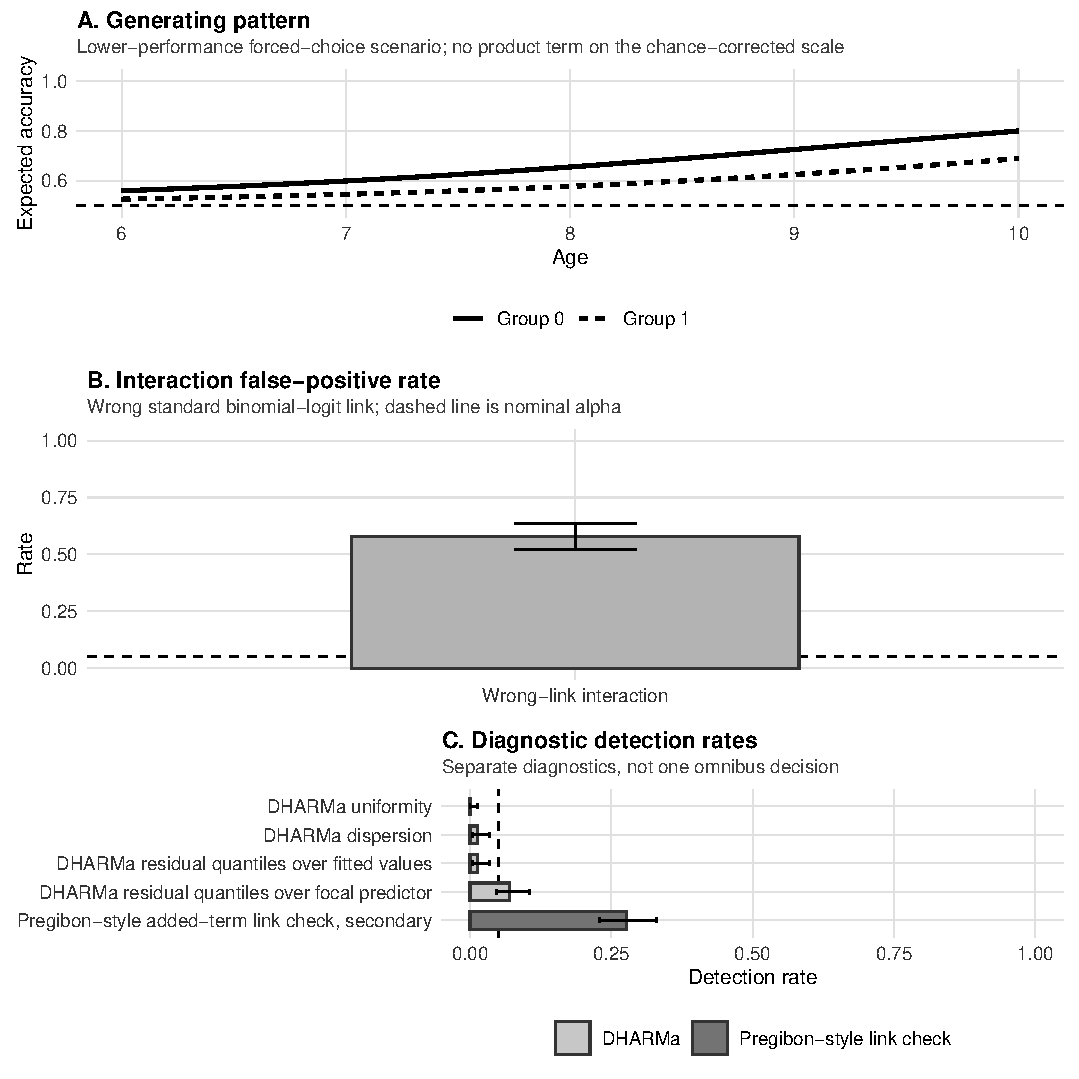
\includegraphics[keepaspectratio]{figs/fig5-diagnostic-worked-example.pdf}}

}

\end{figure}%

The pattern is the one expected from the link-function problem.
Diagnostics help, and AIC can be useful when it compares plausible links
under the same likelihood and the same structural formula. But none of
these tools should be read as a final decision about the scientific
scale of additivity. Residual checks can have limited power, can flag
broad misfit without identifying its source, and can be weakened when
the pseudo-interaction partly absorbs the wrong-link pattern. AIC is a
relative fit comparison among the candidate links supplied by the
analyst, not a proof that the favored link is the scientifically correct
scale. For interaction claims, diagnostics therefore need to be paired
with a clear estimand, a justified link, and sensitivity analyses over
plausible links.

\section{A Minimal Workflow for Link-Aware Interaction
Testing}\label{a-minimal-workflow-for-link-aware-interaction-testing}

The practical implication is not that researchers should stop testing
interactions. It is that interaction claims should be made scale-aware.
A minimal workflow is shown in Table~\ref{tbl-link-aware-workflow}.

\begin{table}

{\caption{{A minimal workflow for link-aware interaction
testing.}{\label{tbl-link-aware-workflow}}}
\vspace{-20pt}}

\begin{longtable}[]{@{}
  >{\raggedright\arraybackslash}p{(\linewidth - 4\tabcolsep) * \real{0.1991}}
  >{\raggedright\arraybackslash}p{(\linewidth - 4\tabcolsep) * \real{0.2832}}
  >{\raggedright\arraybackslash}p{(\linewidth - 4\tabcolsep) * \real{0.5177}}@{}}
\toprule\noalign{}
\begin{minipage}[b]{\linewidth}\raggedright
Step
\end{minipage} & \begin{minipage}[b]{\linewidth}\raggedright
Key question
\end{minipage} & \begin{minipage}[b]{\linewidth}\raggedright
Minimal reporting
\end{minipage} \\
\midrule\noalign{}
\endhead
\bottomrule\noalign{}
\endlastfoot
Define the estimand & What quantity answers the moderation claim? &
State the contrast, moderator values, scale, and whether the estimand is
descriptive, associational, or causal. \\
State the outcome model & What family matches the support and sampling
process? & Report the outcome range, discreteness, trial or item
structure, chance level, and family. \\
Justify the link & On which scale should effects add if there is no
interaction? & Name the link and give the substantive or design reason,
such as odds, latent threshold, log mean, or chance floor. \\
Report the interaction on the relevant scale & Is the claim about the
link scale, the observed scale, or both? & Report predicted means,
contrasts, marginal effects, or difference-in-differences, not only the
product coefficient. \\
Probe robustness & Does the conclusion survive plausible alternatives? &
Report diagnostics and sensitivity analyses across plausible links or
measurement models. \\
\end{longtable}

\end{table}

The workflow is not a rule that makes interaction testing automatic. It
is a compact reporting standard. Researchers still need theory to decide
which contrast matters, which scale is meaningful, and which links are
plausible. The table asks that these decisions be visible before the
product term is interpreted. A linear-predictor coefficient may be
useful for a model-based claim, whereas a response-scale contrast or
marginal effect may be closer to the substantive claim made in words
(\citeproc{ref-mccabe2022}{McCabe et al., 2022};
\citeproc{ref-mize2019}{Mize, 2019}; \citeproc{ref-rohrer2026}{Rohrer \&
Arel-Bundock, 2026}). Diagnostics and predictive checks can warn about
misspecification, but they do not show that the selected link is the
true scientific scale (\citeproc{ref-dunnsmyth1996}{Dunn \& Smyth,
1996}; \citeproc{ref-hartig2024}{Hartig, 2024};
\citeproc{ref-pregibon1980}{Pregibon, 1980}). When the interaction
conclusion is stable across plausible links, the claim becomes easier to
defend. When it is not stable, the conclusion should be stated as
conditional on a modeling choice. This extends a basic reporting
principle: choices that affect the claim should be visible, justified,
and interpretable (\citeproc{ref-mustillo2018}{Mustillo et al., 2018}).

\section{Discussion}\label{discussion}

Interactions remain central to psychological theory, and the point of
this paper is not that they are usually wrong. Some interaction claims
will be stable across reasonable links, scales, and response-scale
summaries. Others will not. Our claim is narrower: many interaction
claims are incomplete unless they state the scale on which additivity,
and therefore no interaction, is being assumed. This scale problem is
well known (\citeproc{ref-cox1984}{Cox, 1984};
\citeproc{ref-loftus1978}{Loftus, 1978};
\citeproc{ref-wagenmakers2012}{Wagenmakers et al., 2012}), but in GLMs
it has a practical form: the link function defines the scale on which
the model is additive. The same issue may also extend beyond
interactions to nonlinear effects, because many psychological analyses
search for curvature, thresholds, and changing slopes without first
specifying the scale on which these patterns are expected
(\citeproc{ref-domingue2024}{Domingue et al., 2024};
\citeproc{ref-mccabe2022}{McCabe et al., 2022};
\citeproc{ref-rohrer2021}{Rohrer \& Arslan, 2021}).

The preregistered review showed why this matters for current practice.
Interaction tests were common, but link functions were often implicit,
and many interaction-testing articles used identity-link analyses in
contexts where the outcome made the scale of additivity worth
justifying. These findings do not show that the reviewed articles
reached false conclusions. They show that the scale of many interaction
claims is difficult to evaluate from the published report.

The conceptual framework separated two modeling problems that are often
mixed together: wrong family and wrong link. It also highlighted a
related measurement problem: the observed score may not be the scale on
which the theoretical interaction claim is meant to hold. These problems
share a common source: psychological constructs are often theorized on
one scale and observed on another. Forced-choice accuracy illustrates
the wrong-link problem clearly. A standard binomial family respects
trial counts, but a standard link may fail to encode the non-zero chance
floor of the task. Sum scores illustrate the measurement-metric problem:
an interaction on the manifest score scale may not be an interaction on
the latent construct scale. Within-family links illustrate the more
general point that even plausible links can define different baselines
for no interaction. In this sense, ordinary floor and ceiling effects
are not a separate problem. They are the visible extreme of a broader
remapping problem that can affect interaction claims even when the
observed data are not obviously piled up at the endpoints.

The simulations were designed to quantify pseudo-interactions, not to
estimate the prevalence of false interactions in the literature. They
show how link and metric choices can generate significant product terms
even when the true interaction is zero on the generating scale. The
diagnostic simulation adds a practical caution. Residual and link checks
can flag some forms of misspecification, and this is useful. But they
rarely answer one clean question, and they should not be read as proof
that an interaction claim is robust to link choice
(\citeproc{ref-dunnsmyth1996}{Dunn \& Smyth, 1996};
\citeproc{ref-hartig2024}{Hartig, 2024};
\citeproc{ref-pregibon1980}{Pregibon, 1980}).

Several limitations are important. First, the review was descriptive and
targeted to selected journals, not a census of psychological research.
Second, we did not code whether published interactions were removable or
nonremovable, because that distinction often cannot be recovered from
published reports alone. Third, the simulations are intentionally
simple. More realistic data may include random effects, item
heterogeneity, lapses, response bias, nonlinear predictors, and missing
data. Fourth, chance-corrected links are appropriate only when a chance
floor is theoretically justified. They are not a universal replacement
for standard binomial models. Finally, logit and probit links often lead
to very similar conclusions, especially away from boundaries; our claim
is that link choice can matter for interaction claims, not that it
always does.

The main contribution is therefore practical. Link-aware interaction
testing does not make moderation claims automatic, and it does not
identify one universally correct scale. It asks researchers to make the
main judgments visible: what outcome family is plausible, what link
defines the no-interaction baseline, what response-scale quantity
answers the substantive question, and whether the conclusion survives
plausible alternatives. This workflow complements existing guidance on
nonlinear interactions, marginal effects, and prediction-based
interpretation (\citeproc{ref-mccabe2022}{McCabe et al., 2022};
\citeproc{ref-mize2019}{Mize, 2019}; \citeproc{ref-rohrer2026}{Rohrer \&
Arel-Bundock, 2026}). When the same conclusion holds across defensible
links, the interaction claim is strengthened. When it changes, the
result can still be informative, but it should be reported as
conditional on a modeling choice. In GLMs, choosing the link is choosing
the scale of the no-interaction claim.

\section{References}\label{references}

\phantomsection\label{refs}
\begin{CSLReferences}{1}{0}
\bibitem[\citeproctext]{ref-ainorton2003}
Ai, C., \& Norton, E. C. (2003). Interaction terms in logit and probit
models. \emph{Economics Letters}, \emph{80}(1), 123--129.
\url{https://doi.org/10.1016/S0165-1765(03)00032-6}

\bibitem[\citeproctext]{ref-burknervuorre2019}
Bürkner, P.-C., \& Vuorre, M. (2019). Ordinal regression models in
psychology: A tutorial. \emph{Advances in Methods and Practices in
Psychological Science}, \emph{2}(1), 77--101.
\url{https://doi.org/10.1177/2515245918823199}

\bibitem[\citeproctext]{ref-cox1984}
Cox, D. R. (1984). Interaction. \emph{International Statistical Review /
Revue Internationale de Statistique}, \emph{52}(1), 1--24.
\url{https://doi.org/10.2307/1403235}

\bibitem[\citeproctext]{ref-czadosantner1992}
Czado, C., \& Santner, T. J. (1992). The effect of link misspecification
on binary regression inference. \emph{Journal of Statistical Planning
and Inference}, \emph{33}(2), 213--231.
\url{https://doi.org/10.1016/0378-3758(92)90069-5}

\bibitem[\citeproctext]{ref-domingue2024}
Domingue, B. W., Kanopka, K., Trejo, S., Rhemtulla, M., \& Tucker-Drob,
E. M. (2024). Ubiquitous bias and false discovery due to model
misspecification in analysis of statistical interactions: The role of
the outcome{'}s distribution and metric properties. \emph{Psychological
Methods}, \emph{29}(6), 1164--1179.
\url{https://doi.org/10.1037/met0000532}

\bibitem[\citeproctext]{ref-dunnsmyth1996}
Dunn, P. K., \& Smyth, G. K. (1996). Randomized quantile residuals.
\emph{Journal of Computational and Graphical Statistics}, \emph{5}(3),
236--244. \url{https://doi.org/10.1080/10618600.1996.10474708}

\bibitem[\citeproctext]{ref-hartig2024}
Hartig, F. (2024). \emph{{DHARMa}: Residual diagnostics for hierarchical
(multi-level / mixed) regression models}.
\url{https://doi.org/10.32614/CRAN.package.DHARMa}

\bibitem[\citeproctext]{ref-liddellkruschke2018}
Liddell, T. M., \& Kruschke, J. K. (2018). Analyzing ordinal data with
metric models: What could possibly go wrong? \emph{Journal of
Experimental Social Psychology}, \emph{79}, 328--348.
\url{https://doi.org/10.1016/j.jesp.2018.08.009}

\bibitem[\citeproctext]{ref-loftus1978}
Loftus, G. R. (1978). On interpretation of interactions. \emph{Memory \&
Cognition}, \emph{6}(3), 312--319.
\url{https://doi.org/10.3758/BF03197461}

\bibitem[\citeproctext]{ref-lubinski1990}
Lubinski, D., \& Humphreys, L. G. (1990). Assessing spurious
{"}moderator effects{"}: Illustrated substantively with the hypothesized
({"}synergistic{"}) relation between spatial and mathematical ability.
\emph{Psychological Bulletin}, \emph{107}(3), 385--393.
\url{https://doi.org/10.1037/0033-2909.107.3.385}

\bibitem[\citeproctext]{ref-mccabe2022}
McCabe, C. J., Halvorson, M. A., King, K. M., Cao, X., \& Kim, D. S.
(2022). Interpreting interaction effects in generalized linear models of
nonlinear probabilities and counts. \emph{Multivariate Behavioral
Research}, \emph{57}(2-3), 243--263.
\url{https://doi.org/10.1080/00273171.2020.1868966}

\bibitem[\citeproctext]{ref-mccullaghnelder1989}
McCullagh, P., \& Nelder, J. A. (1989). \emph{Generalized linear models}
(2nd ed.). Chapman; Hall.

\bibitem[\citeproctext]{ref-micceri1989}
Micceri, T. (1989). The unicorn, the normal curve, and other improbable
creatures. \emph{Psychological Bulletin}, \emph{105}(1), 156--166.

\bibitem[\citeproctext]{ref-mize2019}
Mize, T. D. (2019). Best practices for estimating, interpreting, and
presenting nonlinear interaction effects. \emph{Sociological Science},
\emph{6}, 81--117. \url{https://doi.org/10.15195/v6.a4}

\bibitem[\citeproctext]{ref-mustillo2018}
Mustillo, S. A., Lizardo, O. A., \& McVeigh, R. M. (2018). Editors{'}
Comment: A Few Guidelines for Quantitative Submissions. \emph{American
Sociological Review}, \emph{83}(6), 1281--1283.
\url{https://doi.org/10.1177/0003122418806282}

\bibitem[\citeproctext]{ref-nelderwedderburn1972}
Nelder, J. A., \& Wedderburn, R. W. M. (1972). Generalized linear
models. \emph{Journal of the Royal Statistical Society: Series A
(General)}, \emph{135}(3), 370--384.
\url{https://doi.org/10.2307/2344614}

\bibitem[\citeproctext]{ref-pregibon1980}
Pregibon, D. (1980). Goodness of link tests for generalized linear
models. \emph{Journal of the Royal Statistical Society Series C: Applied
Statistics}, \emph{29}(1), 15--24. \url{https://doi.org/10.2307/2346405}

\bibitem[\citeproctext]{ref-rimpler2026}
Rimpler, A., Kiers, H. A. L., \& Ravenzwaaij, D. van. (2026). Anything
Goes: Statistical Interactions Without Substantive Theory.
\emph{Computational Brain \& Behavior}.
\url{https://doi.org/10.1007/s42113-026-00305-8}

\bibitem[\citeproctext]{ref-rohrer2026}
Rohrer, J. M., \& Arel-Bundock, V. (2026). Models as Prediction
Machines: How to Convert Confusing Coefficients Into Clear Quantities.
\emph{Advances in Methods and Practices in Psychological Science},
\emph{9}(2), 25152459261424825.
\url{https://doi.org/10.1177/25152459261424825}

\bibitem[\citeproctext]{ref-rohrer2021}
Rohrer, J. M., \& Arslan, R. C. (2021). Precise Answers to Vague
Questions: Issues With Interactions. \emph{Advances in Methods and
Practices in Psychological Science}, \emph{4}(2), 25152459211007368.
\url{https://doi.org/10.1177/25152459211007368}

\bibitem[\citeproctext]{ref-smith2020}
Smith, T., Walker, D., \& McKenna, C. (2020). An exploration of link
functions used in ordinal regression. \emph{Journal of Modern Applied
Statistical Methods}, \emph{18}(1).
\url{https://doi.org/10.22237/jmasm/1556669640}

\bibitem[\citeproctext]{ref-stukel1988}
Stukel, T. A. (1988). Generalized logistic models. \emph{Journal of the
American Statistical Association}, \emph{83}(402), 426--431.
\url{https://doi.org/10.1080/01621459.1988.10478613}

\bibitem[\citeproctext]{ref-wagenmakers2012}
Wagenmakers, E.-J., Krypotos, A.-M., Criss, A. H., \& Iverson, G.
(2012). On the interpretation of removable interactions: A survey of the
field 33~years after Loftus. \emph{Memory \& Cognition}, \emph{40}(2),
145--160. \url{https://doi.org/10.3758/s13421-011-0158-0}

\bibitem[\citeproctext]{ref-yuhuang2019}
Yu, S., \& Huang, X. (2019). Link misspecification in generalized linear
mixed models with a random intercept for binary responses. \emph{TEST},
\emph{28}(3), 827--843. \url{https://doi.org/10.1007/s11749-018-0602-6}

\end{CSLReferences}






\end{document}
